\documentclass{article}

%%%%%%%%%%%%%%%%%%%%%%%%%%%%%%%%%%%%%%%%%%%%%%%%%%%%%%%%%%%%%%%%%%%%%
%% Place any additional packages needed here.  Only include packages
%% which are essential, to avoid problems later. Do NOT use any
%% packages which require e-TeX (for example etoolbox): the e-TeX
%% extensions are not currently available on the ACS conversion
%% servers.
%%%%%%%%%%%%%%%%%%%%%%%%%%%%%%%%%%%%%%%%%%%%%%%%%%%%%%%%%%%%%%%%%%%%%
% \usepackage[version=3]{mhchem} % Formula subscripts using \ce{}
\usepackage{siunitx}
\usepackage{tabularx}
\usepackage{float}
\usepackage{booktabs}
\usepackage{amsmath}
\usepackage{amssymb}
\usepackage{amsfonts}
\usepackage{graphicx}
\usepackage{pdflscape}
\usepackage{geometry}
\geometry{a4paper, margin=1in}

\DeclareMathOperator*{\argmax}{arg\,max}
\DeclareMathOperator*{\argmin}{arg\,min}

\title{Supplementary information for Sensitivity test of Markov state models}

\begin{document}
\maketitle

% \begin{figure}
%     \centering
%     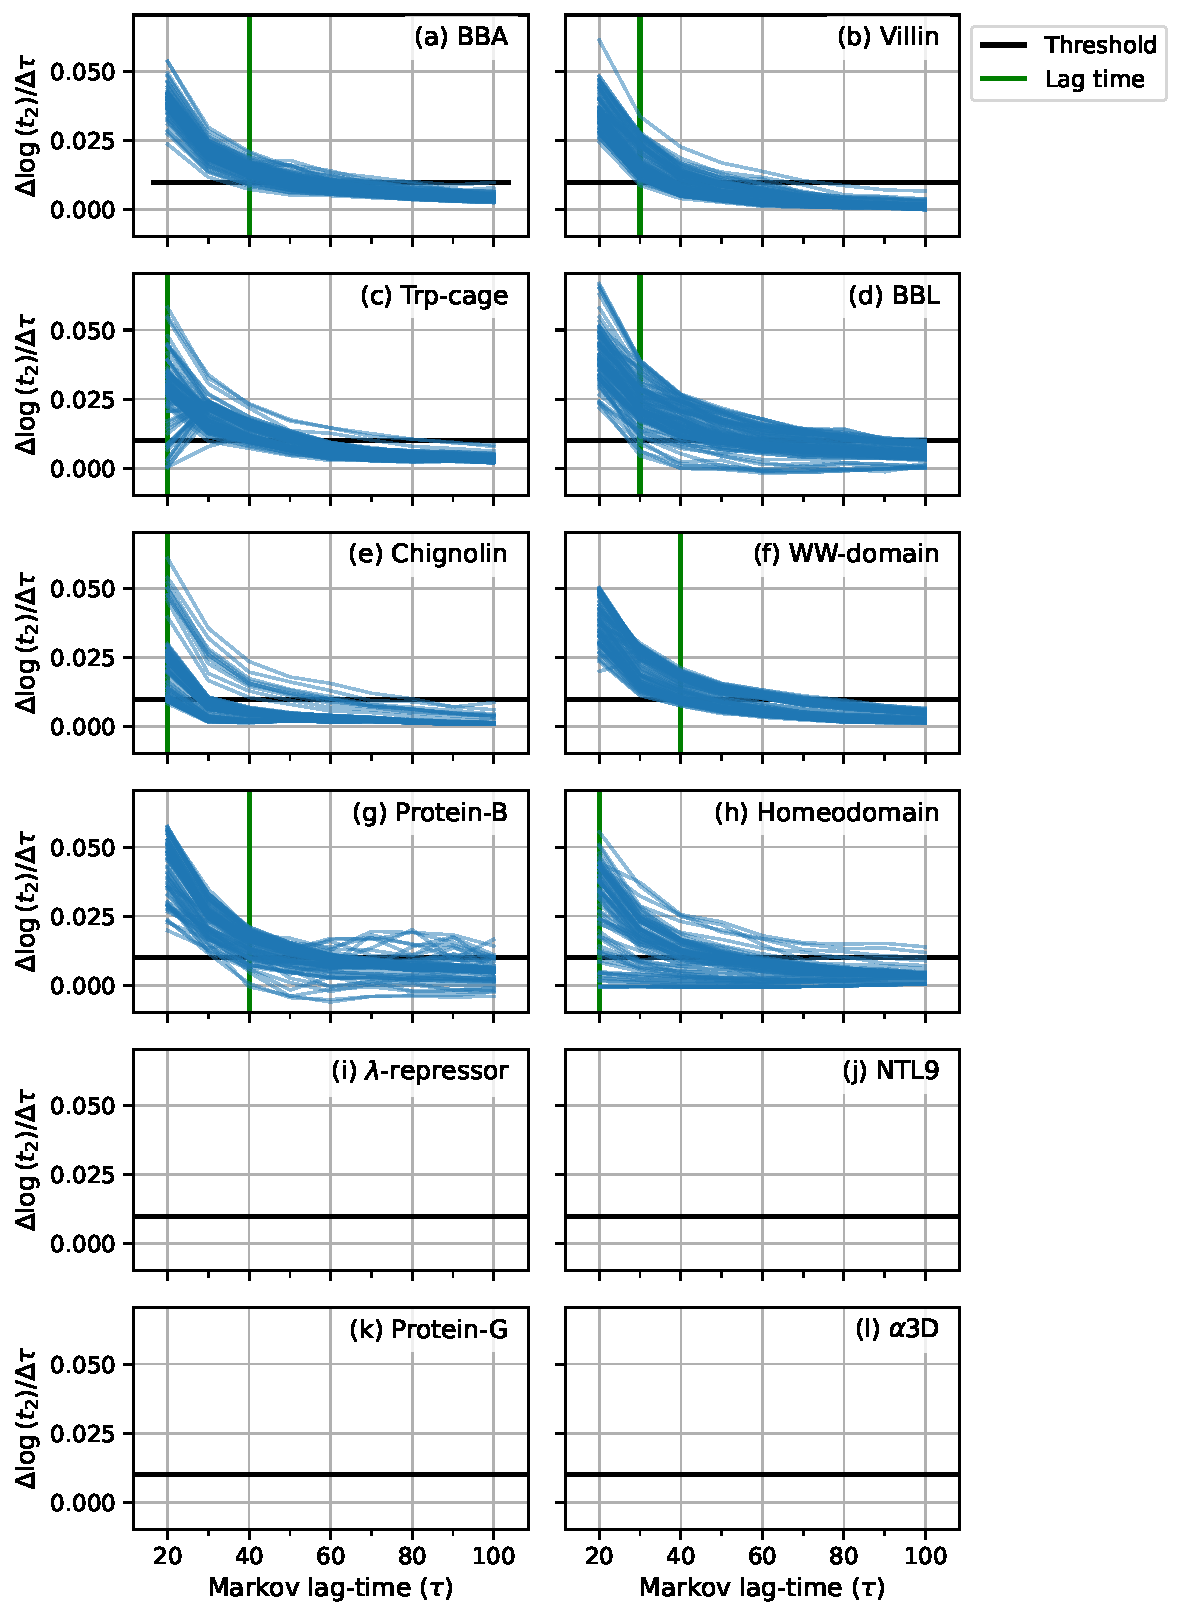
\includegraphics[height=0.65\textheight]{figures/t_2_gradient_sharey_True_log_True_denom_delta_x.pdf}
%     \caption{\textsc{Implied timescale gradient for all hyperparameter trials.} Each panel shows $\Delta \log{\left(t_{2}\right)}/\Delta \tau$: gradient of the dominant timescale ($t_{2}$) with respect to the Markov lag-time. The gradient was calculated for each bootstrap sample and then the median was taken. The horizontal black line is the threshold for determining the lag time. The vertical blue line is the chosen lag-time.}
%     \label{fig:t2_gradient}
% \end{figure}

% \begin{figure}
%     \centering
%     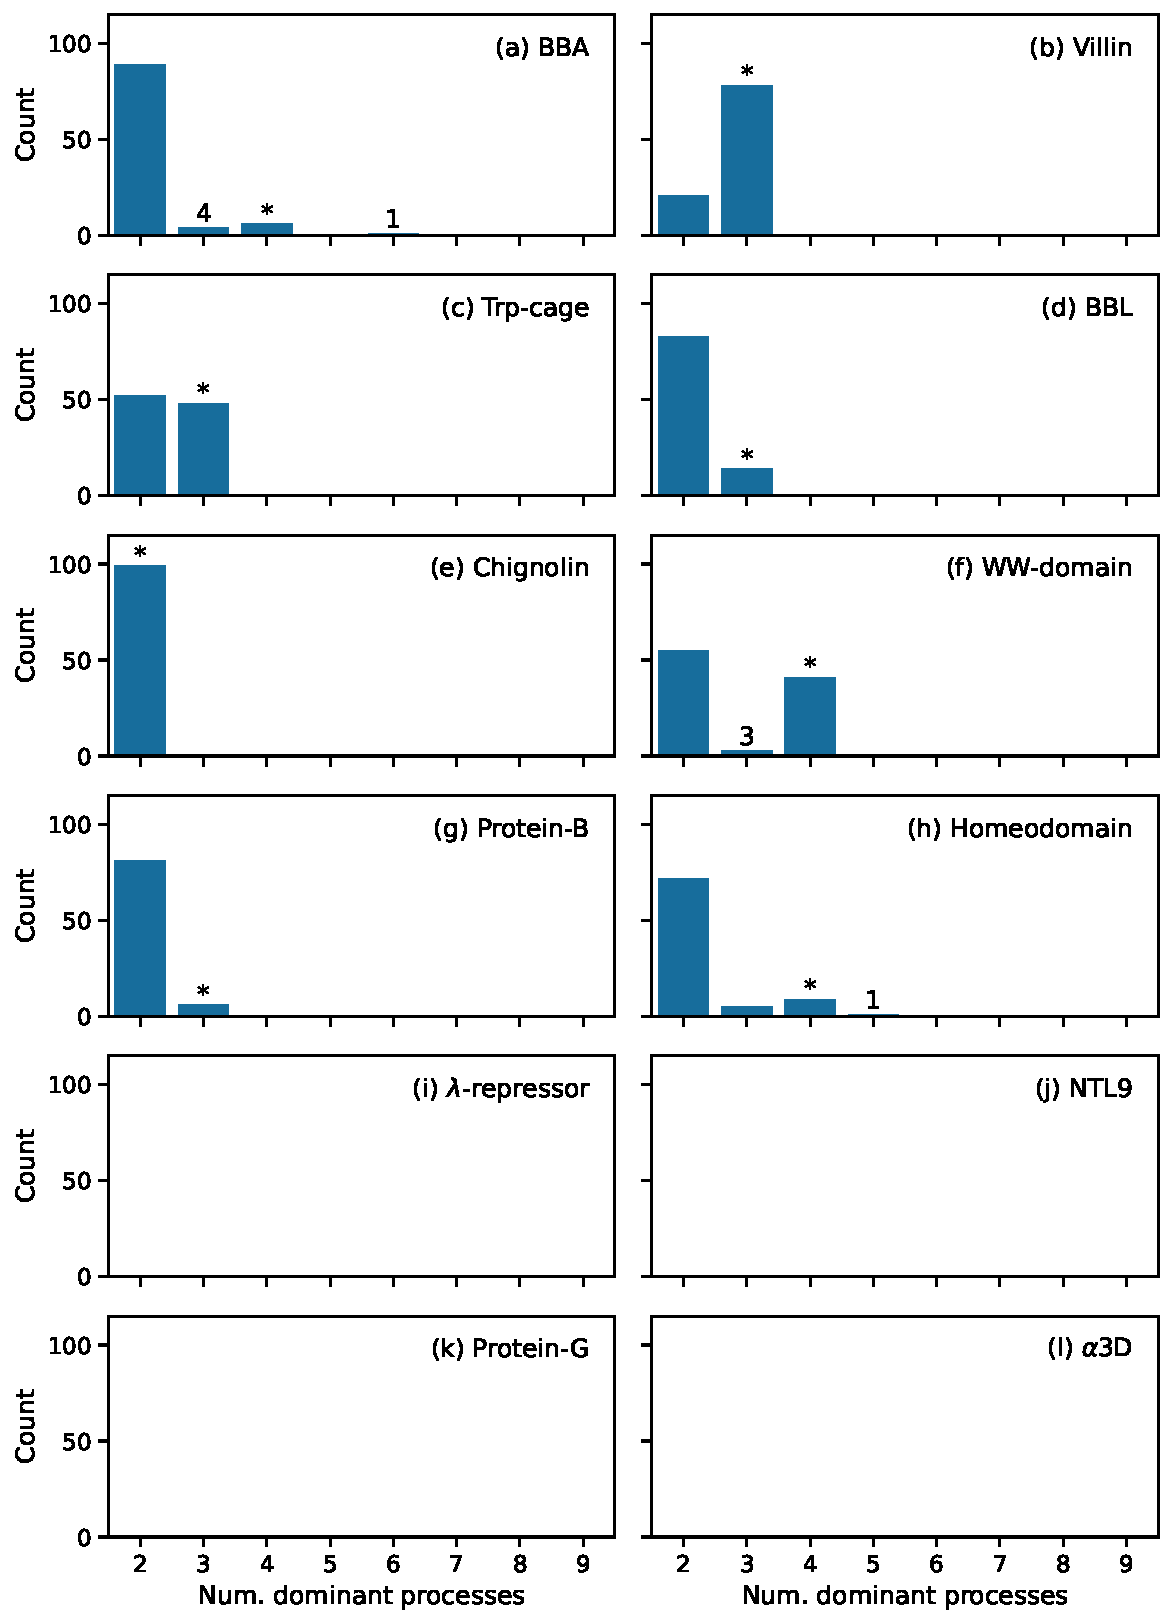
\includegraphics[height=0.6\textheight]{figures/num_dominant_processes_count.pdf}
%     \caption{\textsc{Distribution of the number of dominant process.} For each hyperparameter trial the number of dominant processes was calculated by finding $\argmax_{i}\left[t_{i}/t_{i+1}\right]$ for the $i = 2 - 9$. The selected number of dominant processes was calculated as the largest $i>1$ and is labelled with a `*'.}
%     \label{fig:count_num_proc}
% \end{figure}

\section{Selecting the Markov lag-time}


\begin{figure}
    \centering
    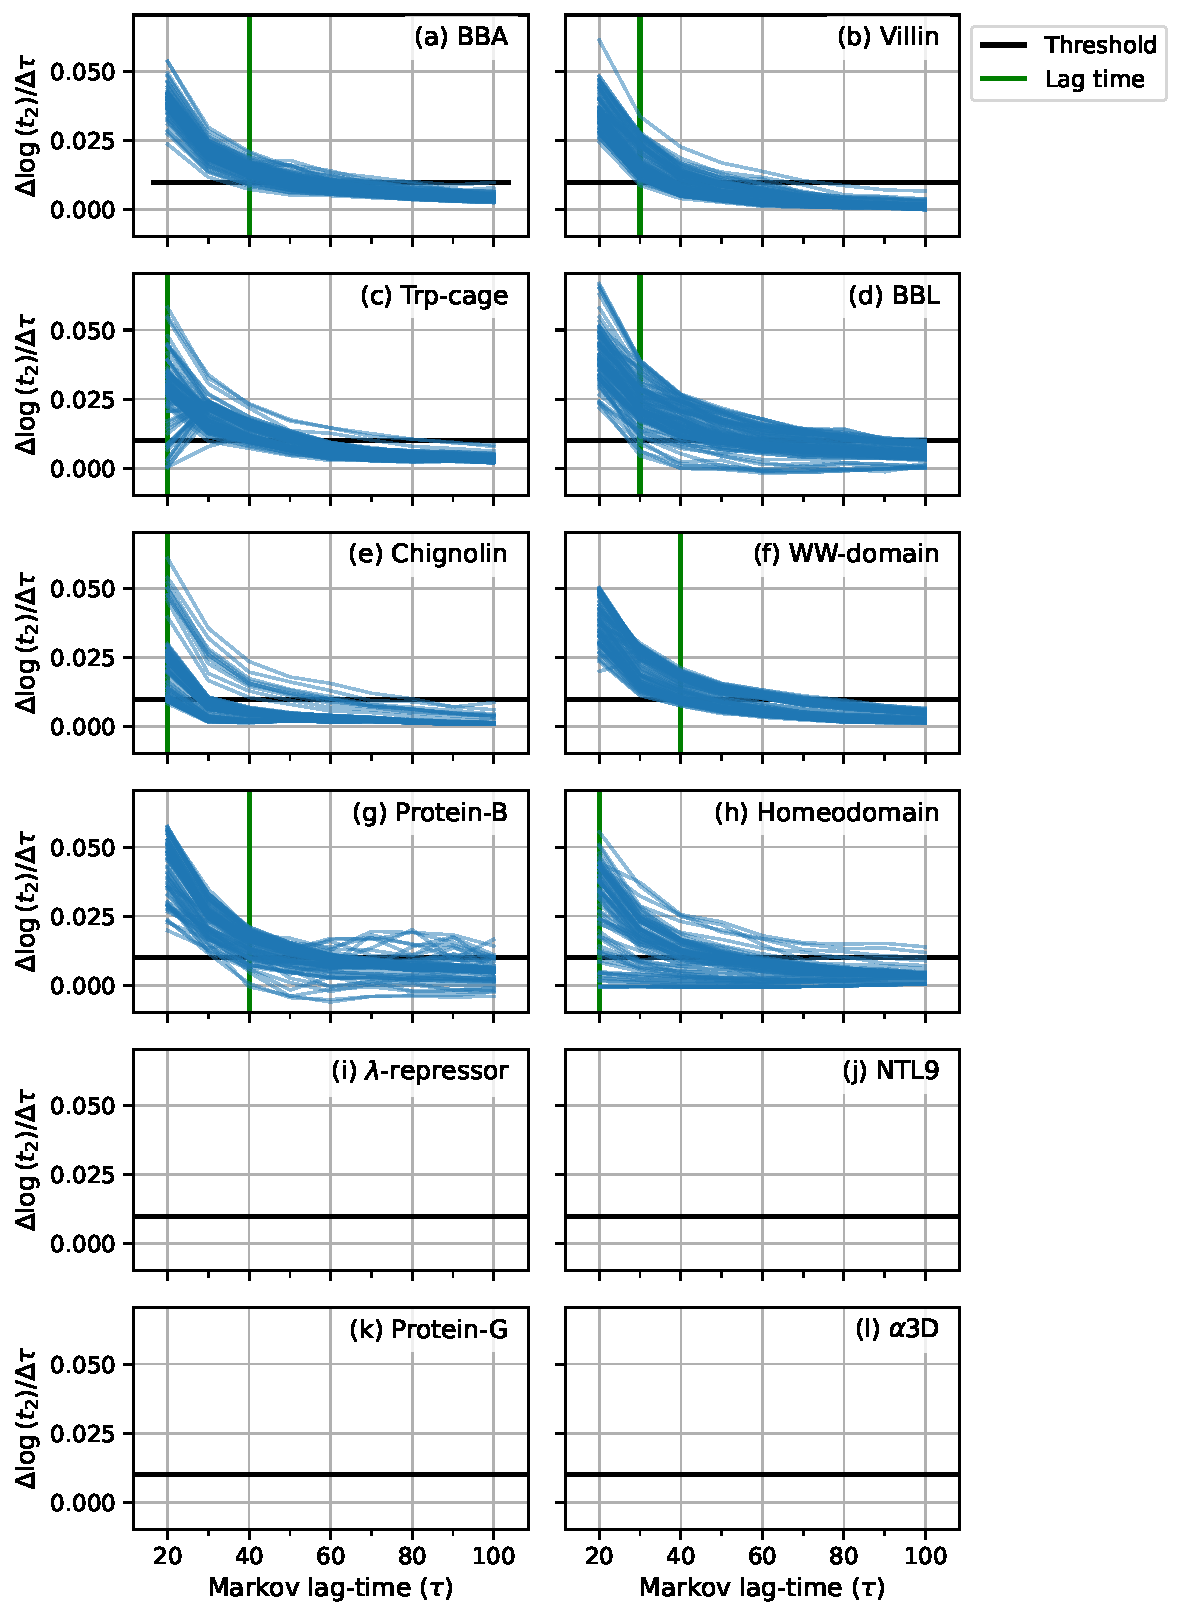
\includegraphics[height=0.8\textheight]{figures/t_2_gradient_sharey_True_log_True_denom_delta_x.pdf}
    \caption{The gradient of the implied timescales for each trial for each protein.  Each blue line is the gradient of the logarithm of the the second (i.e., longest) implied timescale for each hyperparameter trial, calculated as the median over \num{100} bootstrap samples. The black horizontal line is the threshold for convergence. The green vertical is the selected Markov lag time calculated as the smallest lag time at which a single trial crosses the threshold.}
    \label{fig:its_grad_all}
\end{figure}

\begin{figure}
    \centering
    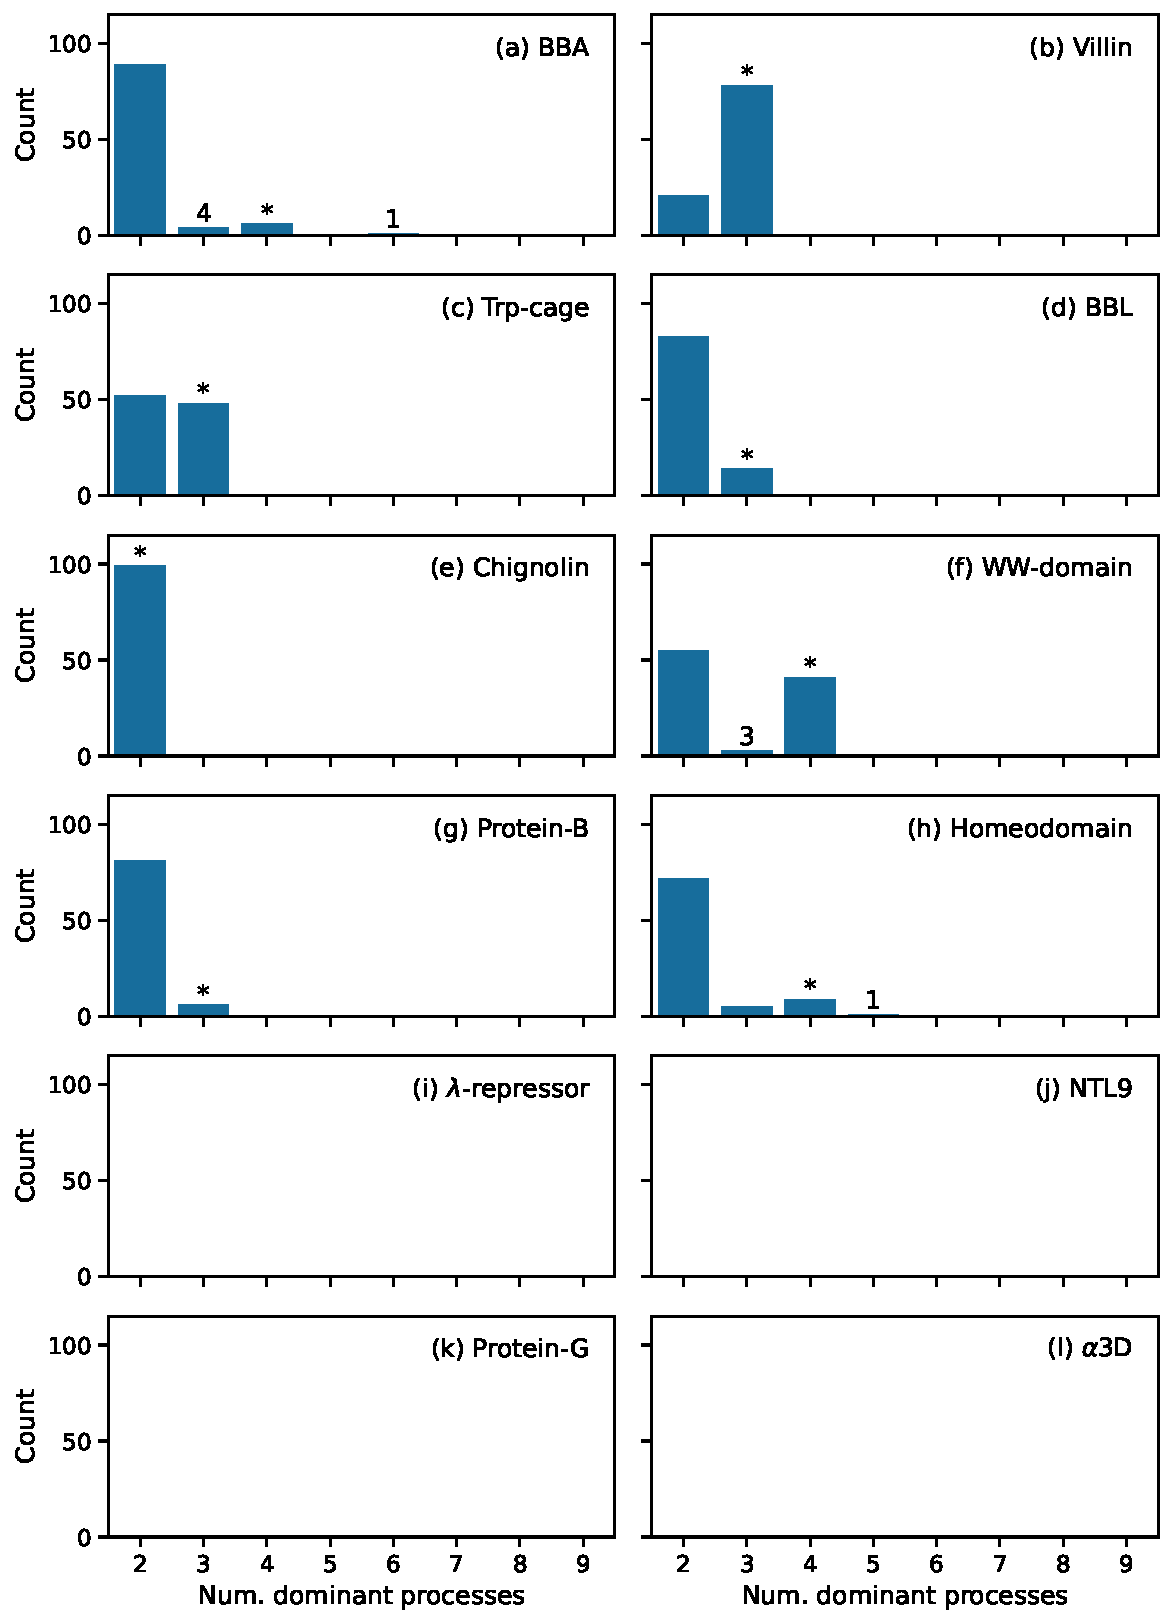
\includegraphics[height=0.8\textheight]{figures/num_dominant_processes_count.pdf}
    \caption{The distribution of dominant timescales for each protein.  The number of dominant timescales are the number of timescales which lie above the largest timescale gap ($t_{i}/t_{i+1}$). The selected number of timescales are shown with an asterisk ('*') and are calculated as the largest number of timescales which have two or more trials with that number.}
    \label{fig:num_proc_all}
\end{figure}

\section{BBA}



% \begin{landscape}

% \begin{table}
% \begin{tabular}{llllllll}
% \toprule
% Model no. &                  1 &                  2 &                  3 &                  4 &                  5 &                  6 &                  7 \\
% \midrule
% Method                         &          Fixed $k$ &          Fixed $k$ &          Fixed $k$ &  Fixed $k$ (worst) &             TS Gap &             TS Gap &             TS Gap \\
% Lag (ns)                       &                 40 &                 40 &                 40 &                 40 &                 40 &                 40 &                 40 \\
% Feature                        &          Dihedrals &          Distances &          Distances &          Distances &          Dihedrals &          Distances &          Distances \\
% Transform                      &                  - &           Logistic &             Linear &           Logistic &                  - &             Linear &           Logistic \\
% Contact scheme                 &                  - &          C$\alpha$ &          C$\alpha$ &      Closest-Heavy &                  - &      Closest-Heavy &          C$\alpha$ \\
% Center (\si{\angstrom})        &                  - &                6.1 &                  - &               13.3 &                  - &                  - &                4.7 \\
% Steepness (\si{\per\angstrom}) &                  - &                2.5 &                  - &                1.7 &                  - &                  - &                0.5 \\
% TICA lag (ns)                  &                 45 &                 63 &                 84 &                 87 &                 19 &                 13 &                 16 \\
% TICA dimension                 &                  9 &                  6 &                 10 &                  1 &                  1 &                  2 &                  1 \\
% Num. clusters                  &                291 &                349 &                260 &                 96 &                220 &                413 &                392 \\
% $k_{\mathrm{fixed}}$           &                  4 &                  4 &                  4 &                  4 &                  4 &                  4 &                  4 \\
% $k_{\mathrm{gap}}$             &                  2 &                  2 &                  2 &                  2 &                  2 &                  2 &                  2 \\
% VAMP-2(k=2)                    &  1.95, [1.94-1.96] &  1.97, [1.95-1.98] &  1.97, [1.95-1.98] &  1.92, [1.91-1.94] &  1.96, [1.95-1.97] &  1.96, [1.96-1.97] &  1.96, [1.95-1.97] \\
% VAMP-2(k=3)                    &  2.86, [2.80-2.90] &  2.93, [2.90-2.95] &  2.93, [2.90-2.95] &  2.36, [2.31-2.40] &  2.57, [2.54-2.60] &  2.80, [2.74-2.91] &  2.70, [2.63-2.89] \\
% VAMP-2(k=4)                    &  3.72, [3.63-3.81] &  3.88, [3.84-3.91] &  3.87, [3.83-3.90] &  2.51, [2.44-2.56] &  3.01, [2.93-3.09] &  3.57, [3.41-3.72] &  3.37, [3.16-3.58] \\
% \bottomrule
% \end{tabular}
% \caption{\textsc{Summary of comparator models for BBA.} Models 1 - 4 are selected using a fixed number of processes ($k_{\mathrm{fixed}}$) in the VAMP2 score, and are the best performing models for each feature (1 -3) and the worst performing model overall (4).  Models 5 - 7 are the best performing models for each feature after consideration of the timescale gap. The number of processes is used to calculate this is $k_{\mathrm{gap}}$.}
% \label{tab:1fme_mod_defs}
% \end{table}
% \end{landscape}

% \clearpage
% \subsection{VAMP-2 scores}

% \begin{figure}[h]
%     \centering
%     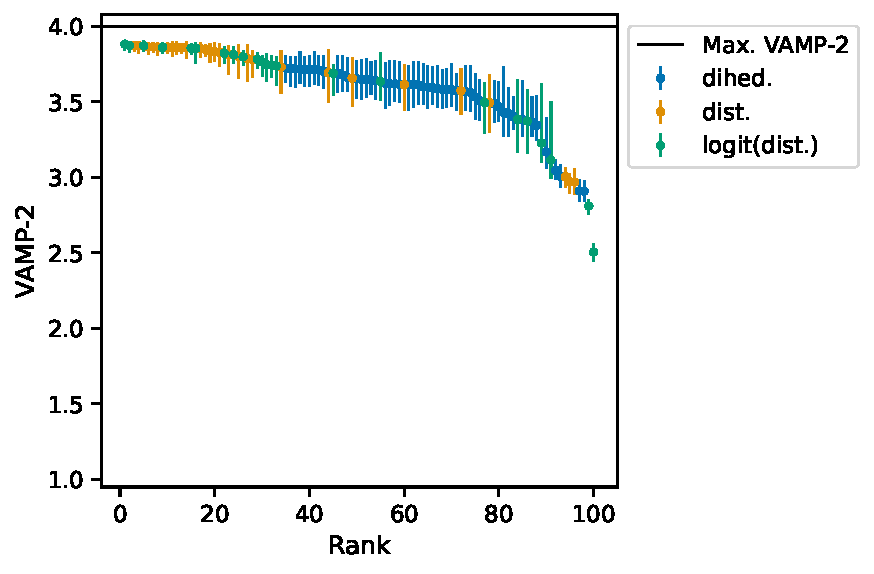
\includegraphics[width=0.9\textwidth]{figures/vamp_scores/BBA_vamp_scores_ranked.pdf}
%     \caption{BBA hyperparameter trial scores using the VAMP-2 with $k=4$ eigenvectors. Trials are ranked using the median of the VAMP-2 score, errors shown are the \SI{95}{\percent} quantiles of 100 bootstrapped estimates.}
%     \label{fig:bba_vamp_fixed_k}
% \end{figure}

% \clearpage
% \begin{figure}
%     \centering
%     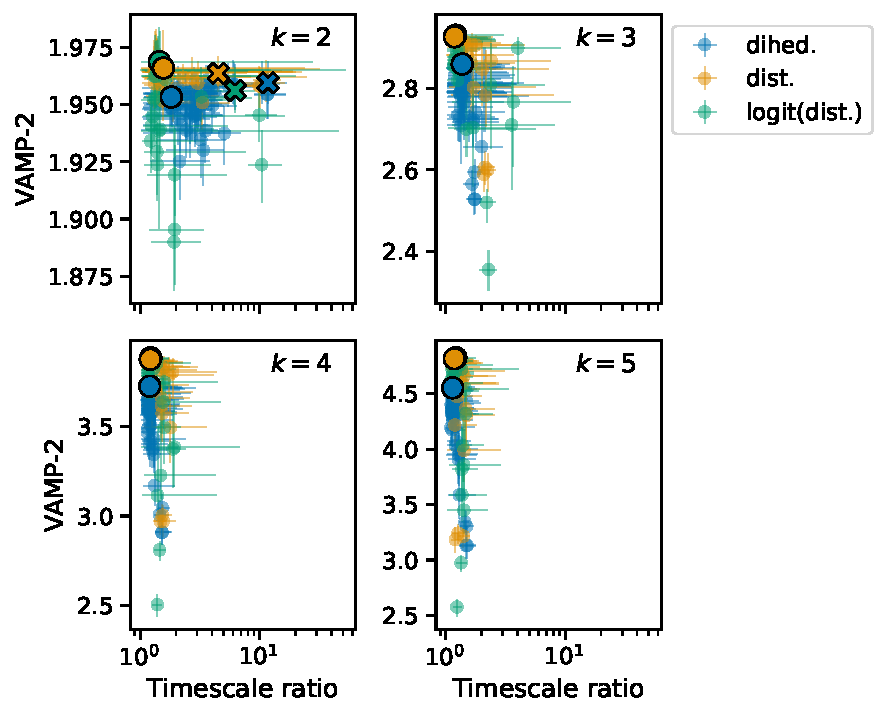
\includegraphics[width=0.9\textwidth]{figures/vamp_scores/BBA_vamp_vs_gap.pdf}
%     \caption{BBA hyperparameter trial scores and implied timescale gaps.  Each panel shows the VAMP-2 score with $k$ eigenvectors against the ratio of implied timescales $t_{k}/t_{k+1}$. Large coloured disks show the models selected using $k=4$ eigenvectors (models 1 - 3 in table \ref{tab:1fme_mod_defs}).  Crosses show the models selected using the timescale ratio and VAMP-2 scores (models 5 - 7 in table \ref{tab:1fme_mod_defs}).}
%     \label{fig:bba_vamp_var_k}
% \end{figure}


% \clearpage
% \subsection{Chapman-Kolmogorov Tests}

% \begin{figure}[h]
%     \centering
%     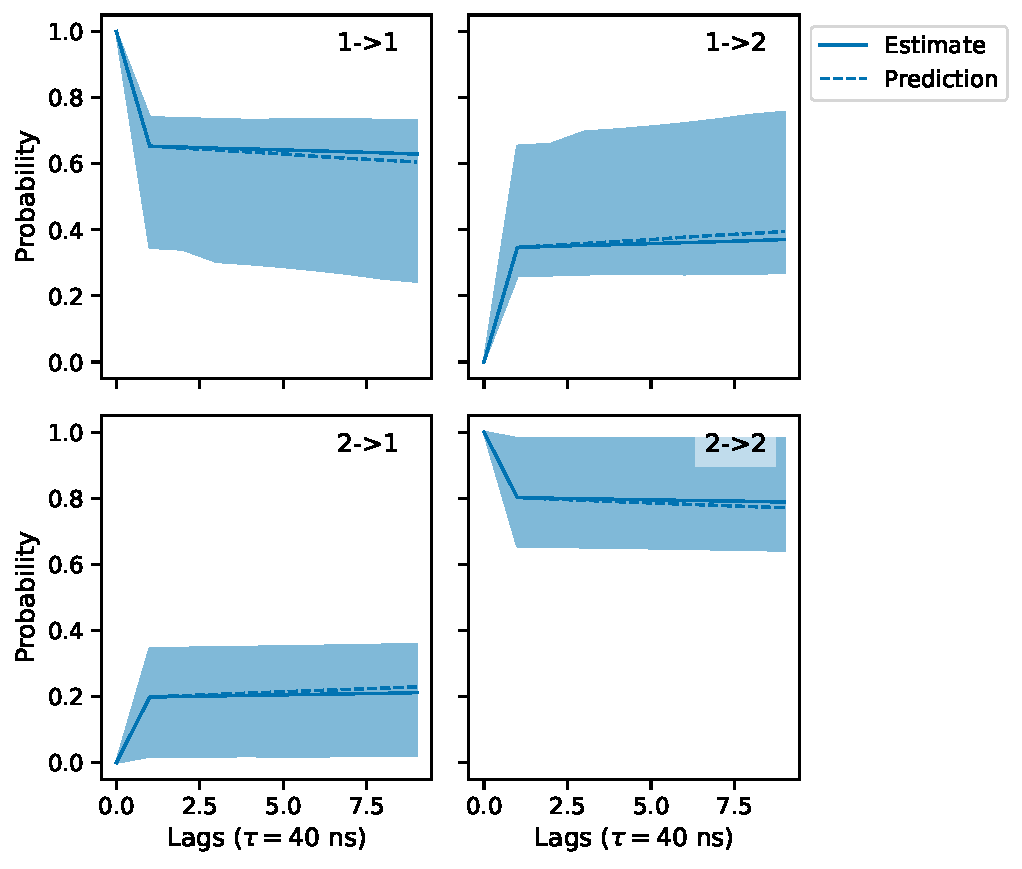
\includegraphics[height=0.4\textheight]{figures/cktests/bba/m1_dihed_hpix47_cktest.pdf}
%     \caption{Chapman Kolmogorov test for BBA model 1 (table \ref{tab:1fme_mod_defs}). Estimate and errors are the median and \SI{95}{\percent} bootstrapped quantiles respectively.}
%     \label{fig:cktest_bba_1}
% \end{figure}

% \begin{figure}
%     \centering
%     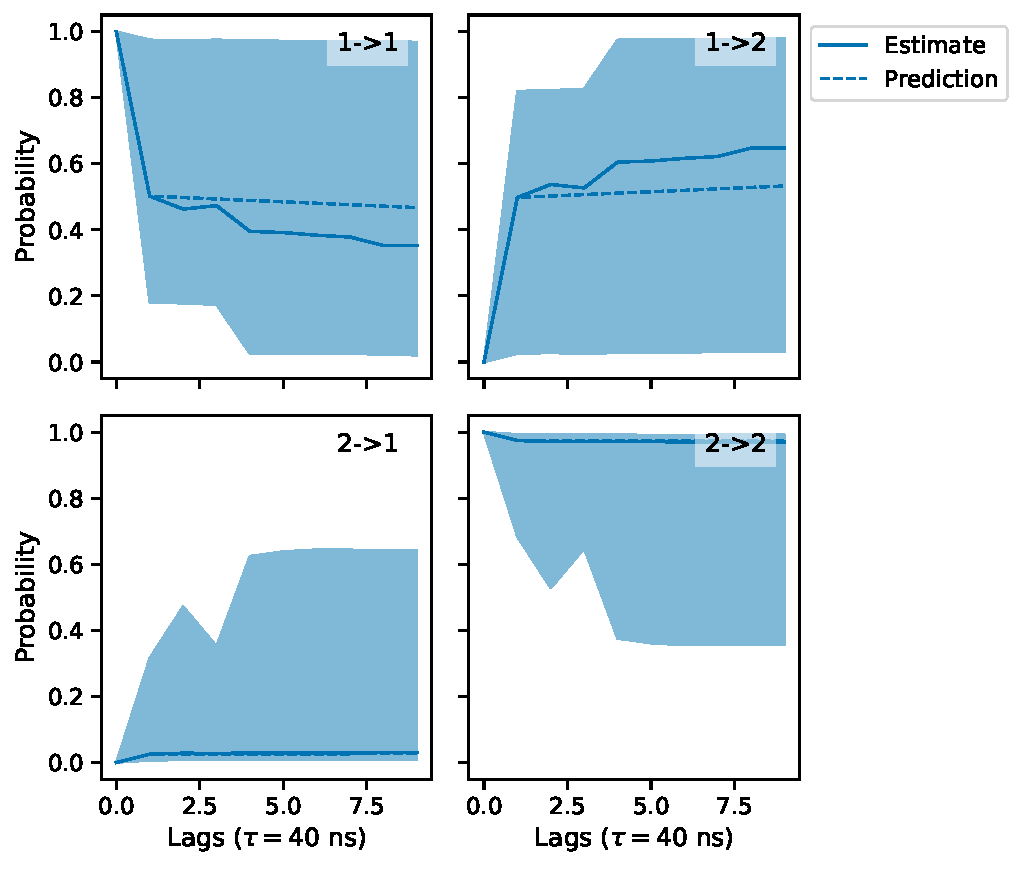
\includegraphics[height=0.4\textheight]{figures/cktests/bba/m1_logit(dist)_hpix81_cktest.pdf}
%     \caption{Chapman Kolmogorov test for BBA model 2 (table \ref{tab:1fme_mod_defs}). Estimate and errors are the median and \SI{95}{\percent} bootstrapped quantiles respectively. }
%     \label{fig:cktest_bba_2}
% \end{figure}

% \begin{figure}
%     \centering
%     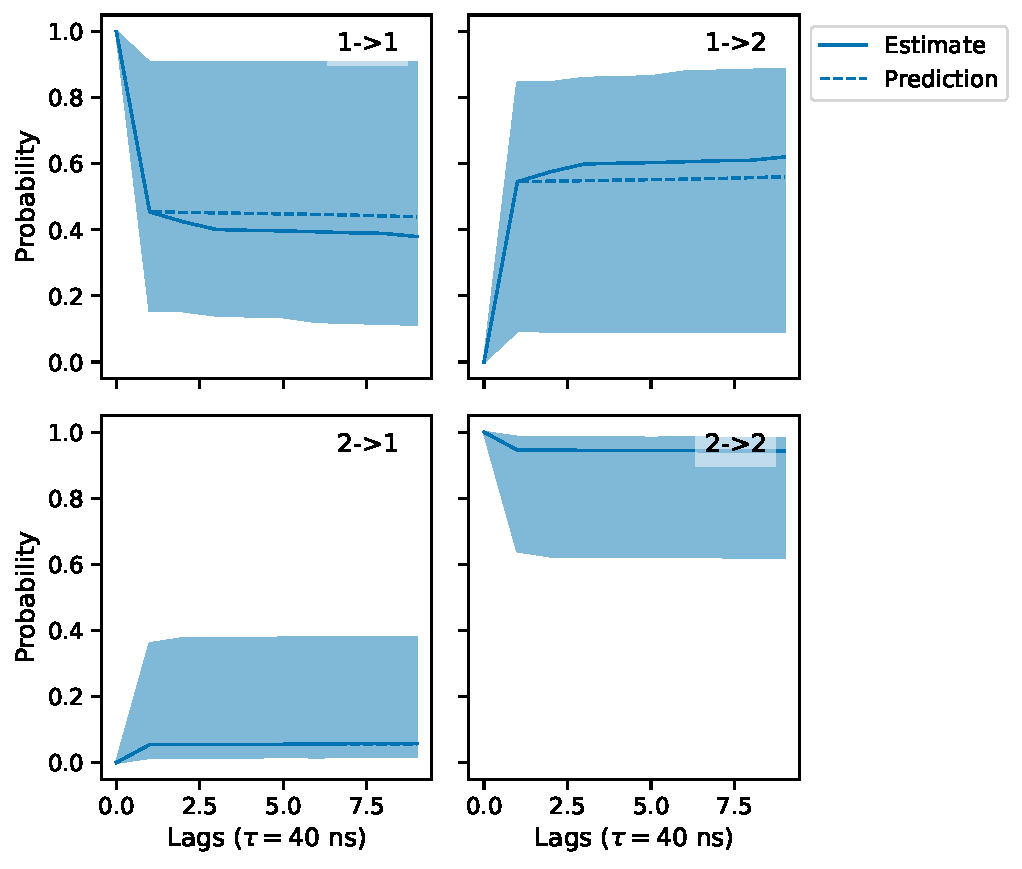
\includegraphics[height=0.4\textheight]{figures/cktests/bba/m1_dist_hpix99_cktest.pdf}
%     \caption{Chapman Kolmogorov test for BBA model 3 (table \ref{tab:1fme_mod_defs}). Estimate and errors are the median and \SI{95}{\percent} bootstrapped quantiles respectively.}
%     \label{fig:cktest_bba_3}
% \end{figure}

% \begin{figure}
%     \centering
%     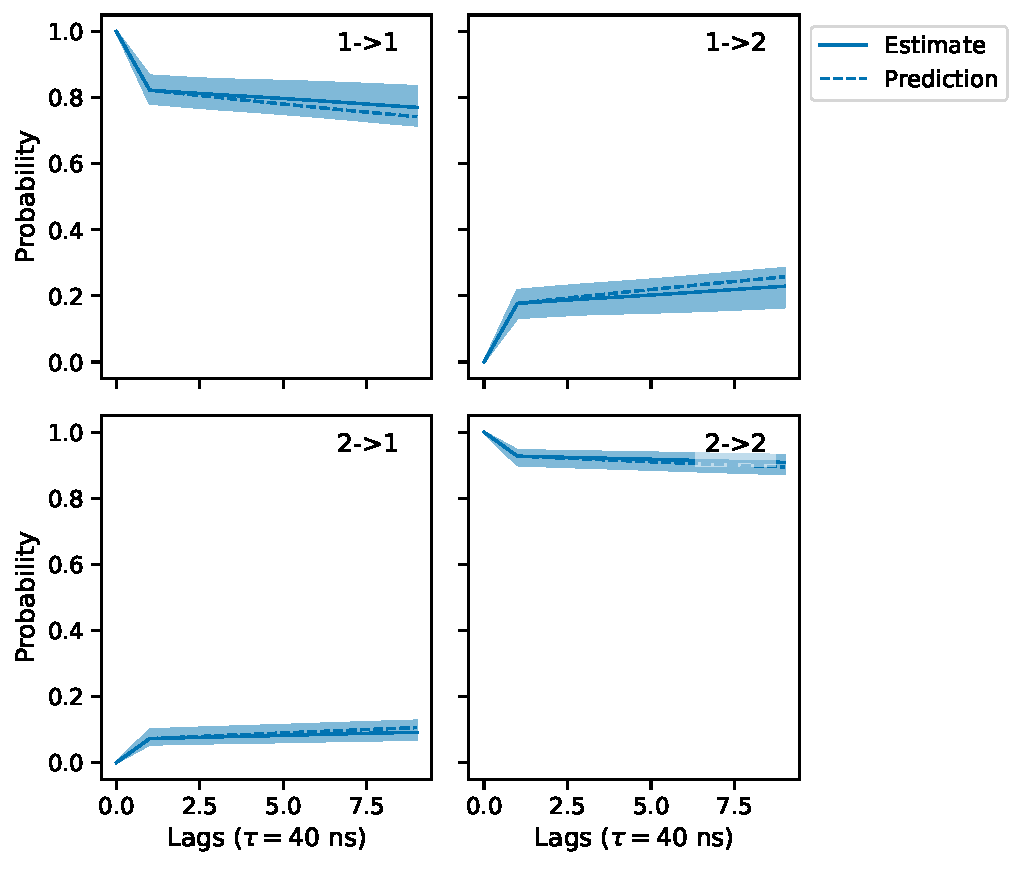
\includegraphics[height=0.4\textheight]{figures/cktests/bba/m2_dihed_hpix30_cktest.pdf}
%     \caption{Chapman Kolmogorov test for BBA model 5 (table \ref{tab:1fme_mod_defs}). Estimate and errors are the median and \SI{95}{\percent} bootstrapped quantiles respectively.}
%     \label{fig:cktest_bba_5}
% \end{figure}

% \begin{figure}
%     \centering
%     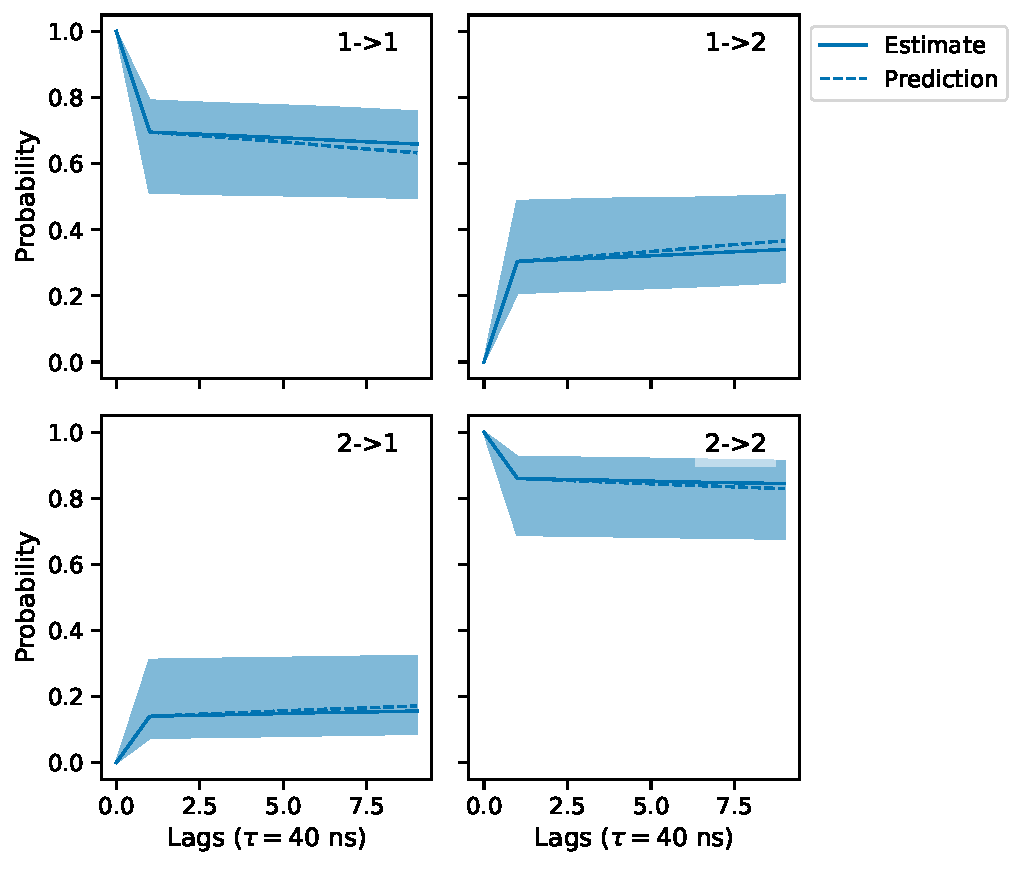
\includegraphics[height=0.4\textheight]{figures/cktests/bba/m2_logit(dist)_hpix91_cktest.pdf}
%     \caption{Chapman Kolmogorov test for BBA model 6 (table \ref{tab:1fme_mod_defs}). Estimate and errors are the median and \SI{95}{\percent} bootstrapped quantiles respectively.}
%     \label{fig:cktest_bba_6}
% \end{figure}

% \begin{figure}
%     \centering
%     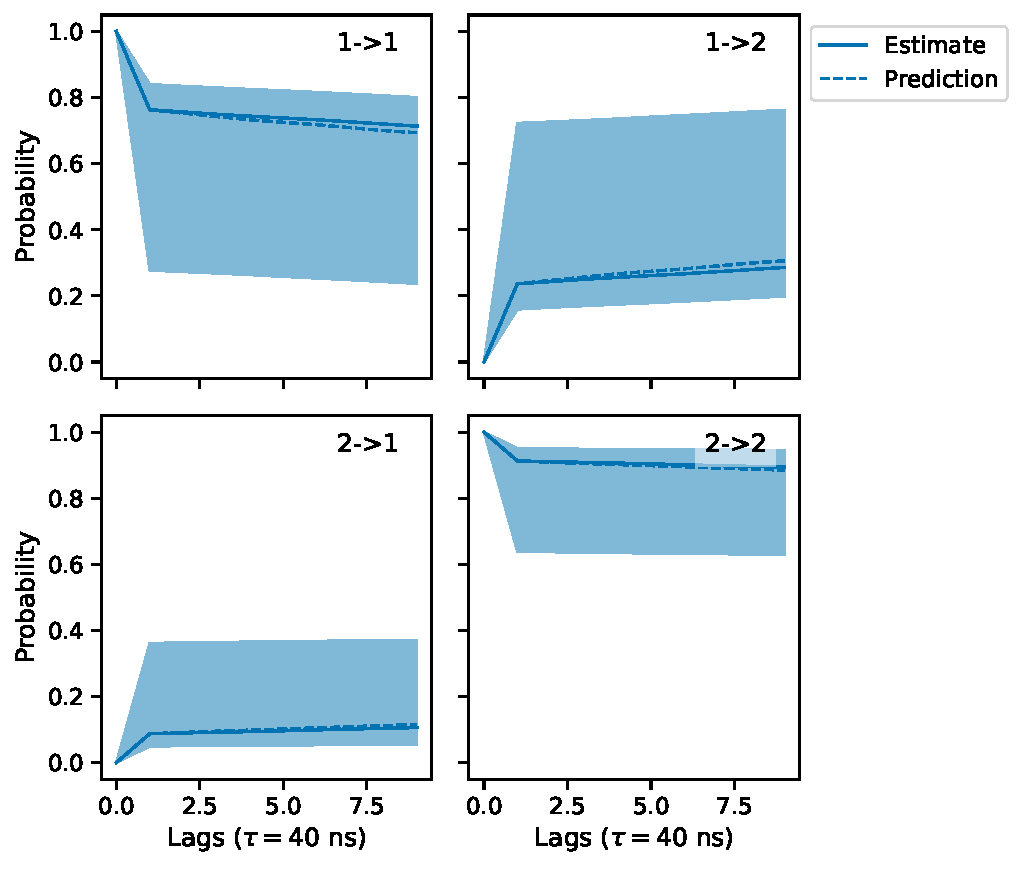
\includegraphics[height=0.4\textheight]{figures/cktests/bba/m2_dist_hpix27_cktest.pdf}
%     \caption{Chapman Kolmogorov test for BBA model 7 (table \ref{tab:1fme_mod_defs}). Estimate and errors are the median and \SI{95}{\percent} bootstrapped quantiles respectively.}
%     \label{fig:cktest_bba_7}
% \end{figure}

% \clearpage
% \subsection{Implied timescales and separation of timescales}

% \begin{figure}[h]
%     \centering
%     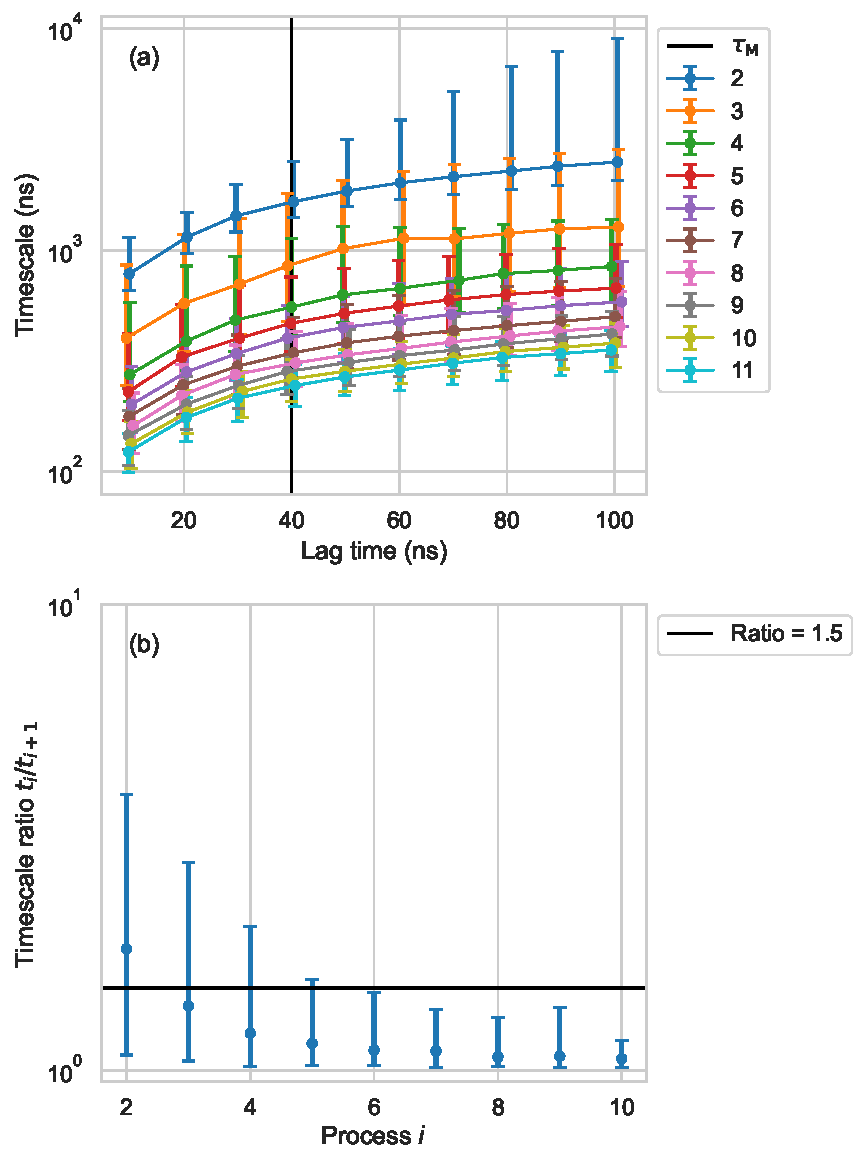
\includegraphics[height=0.65\textheight]{figures/its/bba/BBA_model_dihed._method_m1.pdf}
%     \caption{Implied timescales (panel (a)) and ratios of implied timescales at $\tau=\SI{40}{\nano\second}$ (panel (b)) for BBA model 1 (table \ref{tab:1fme_mod_defs}). Estimate and errors are the median and \SI{95}{\percent} bootstrapped quantiles respectively.}
%     \label{fig:its_bba_1}
% \end{figure}

% \begin{figure}
%     \centering
%     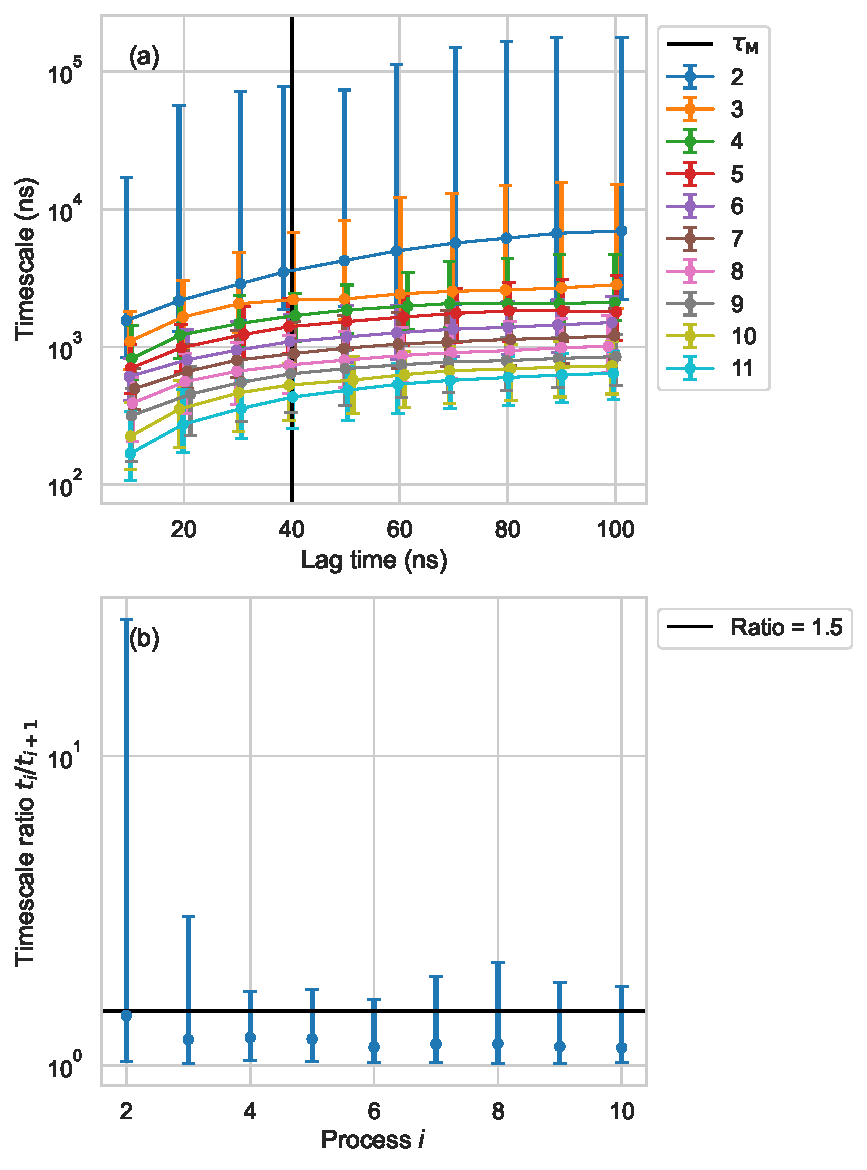
\includegraphics[height=0.65\textheight]{figures/its/bba/BBA_model_logit(dist.)_method_m1.pdf}
%     \caption{Implied timescales (panel (a)) and ratios of implied timescales at $\tau=\SI{40}{\nano\second}$ (panel (b)) for BBA model 2 (table \ref{tab:1fme_mod_defs}). Estimate and errors are the median and \SI{95}{\percent} bootstrapped quantiles respectively.}
%     \label{fig:its_bba_2}
% \end{figure}

% \begin{figure}
%     \centering
%     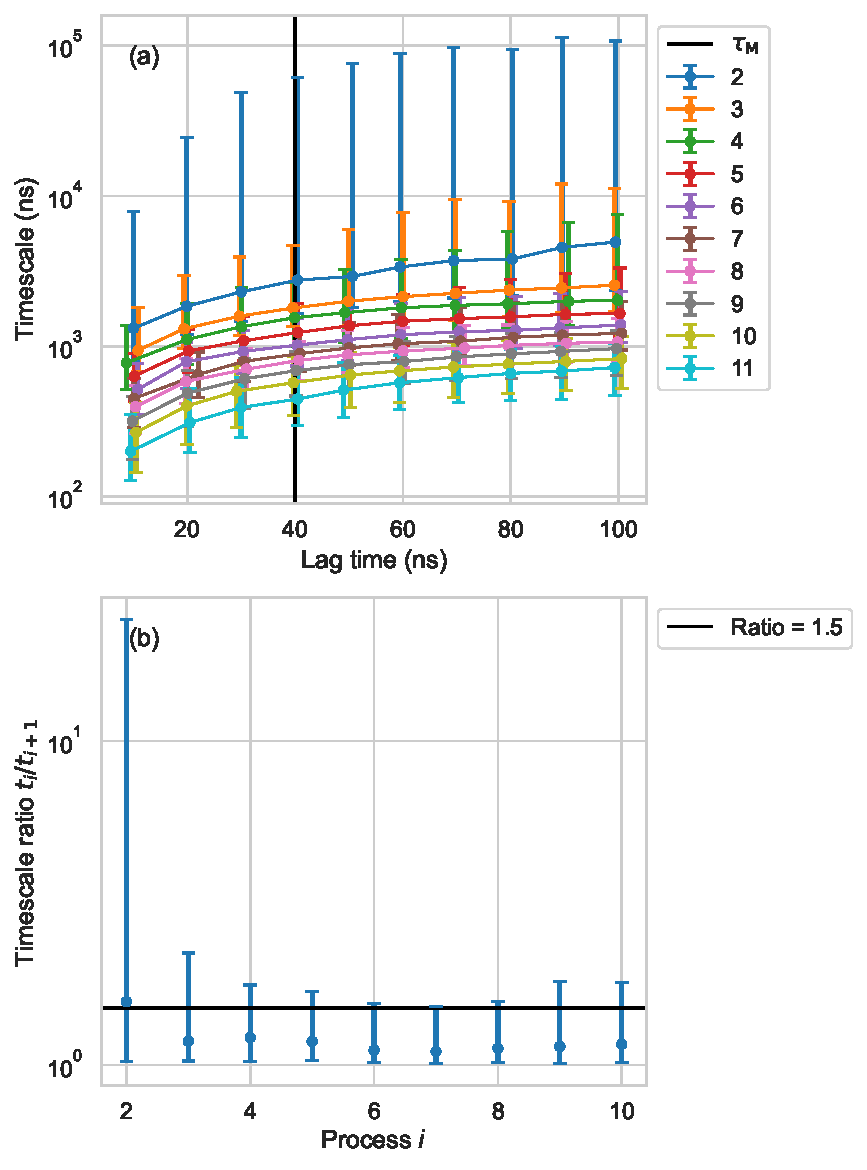
\includegraphics[height=0.65\textheight]{figures/its/bba/BBA_model_dist._method_m1.pdf}
%     \caption{Implied timescales (panel (a)) and ratios of implied timescales at $\tau=\SI{40}{\nano\second}$ (panel (b)) for BBA model 3 (table \ref{tab:1fme_mod_defs}). Estimate and errors are the median and \SI{95}{\percent} bootstrapped quantiles respectively.}
%     \label{fig:its_bba_3}
% \end{figure}

% \begin{figure}
%     \centering
%     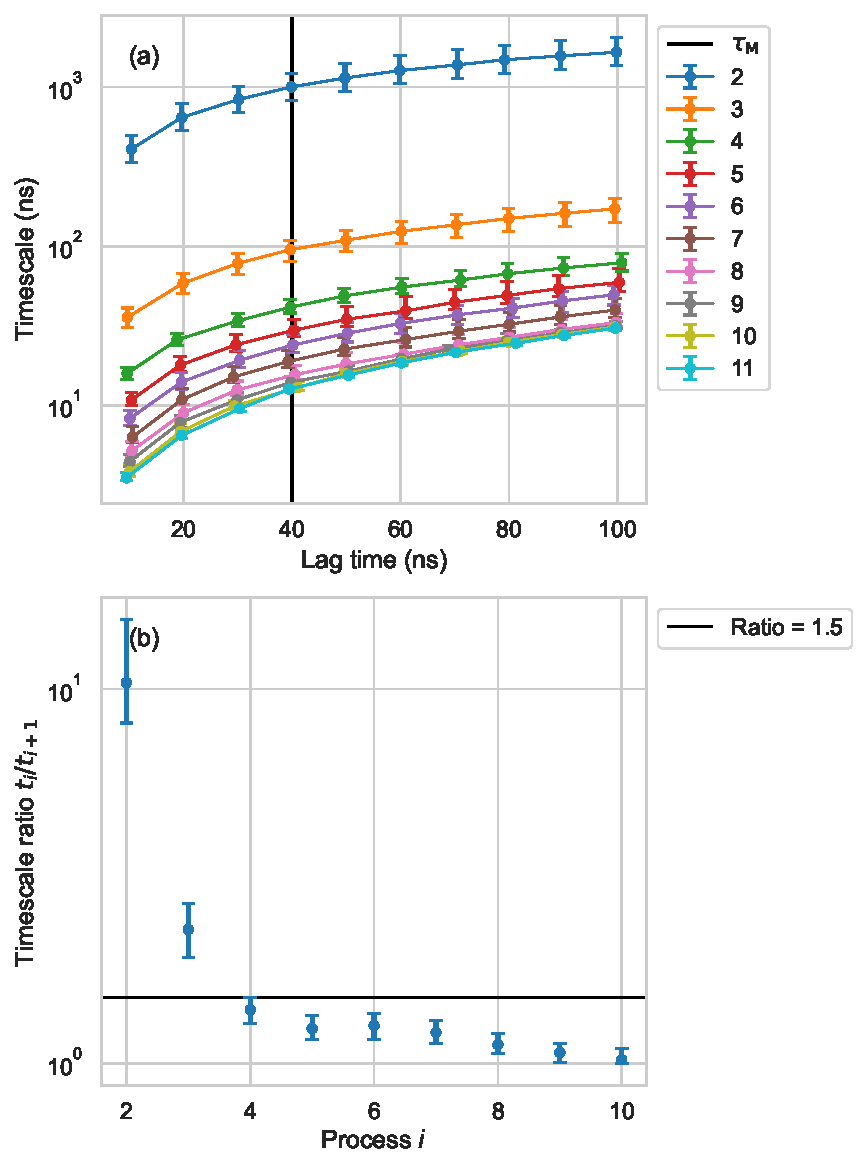
\includegraphics[height=0.65\textheight]{figures/its/bba/BBA_model_logit(dist.)_method_m3.pdf}
%     \caption{Implied timescales (panel (a)) and ratios of implied timescales at $\tau=\SI{40}{\nano\second}$ (panel (b)) for BBA model 4 (table \ref{tab:1fme_mod_defs}). Estimate and errors are the median and \SI{95}{\percent} bootstrapped quantiles respectively.}
%     \label{fig:its_bba_4}
% \end{figure}

% \begin{figure}
%     \centering
%     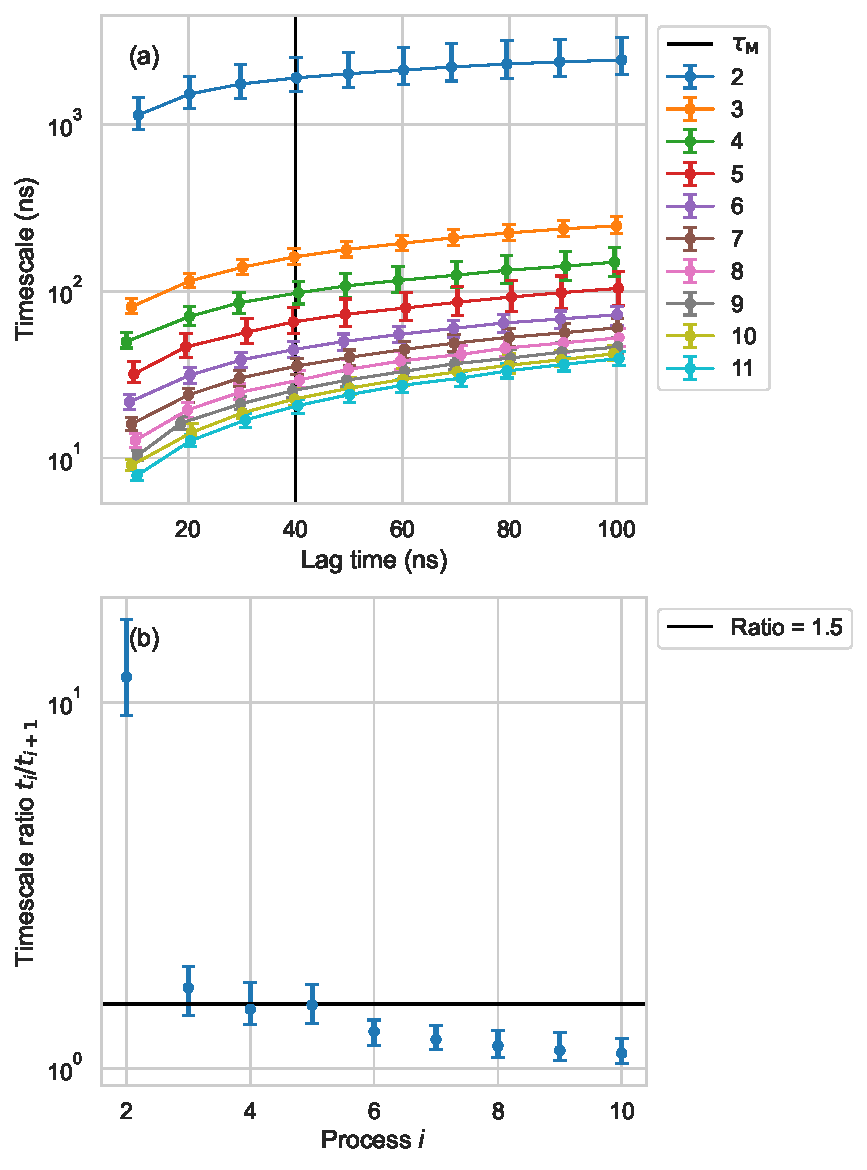
\includegraphics[height=0.65\textheight]{figures/its/bba/BBA_model_dihed._method_m2.pdf}
%     \caption{Implied timescales (panel (a)) and ratios of implied timescales at $\tau=\SI{40}{\nano\second}$ (panel (b)) for BBA model 5 (table \ref{tab:1fme_mod_defs}). Estimate and errors are the median and \SI{95}{\percent} bootstrapped quantiles respectively.}
%     \label{fig:its_bba_5}
% \end{figure}



% \begin{figure}
%     \centering
%     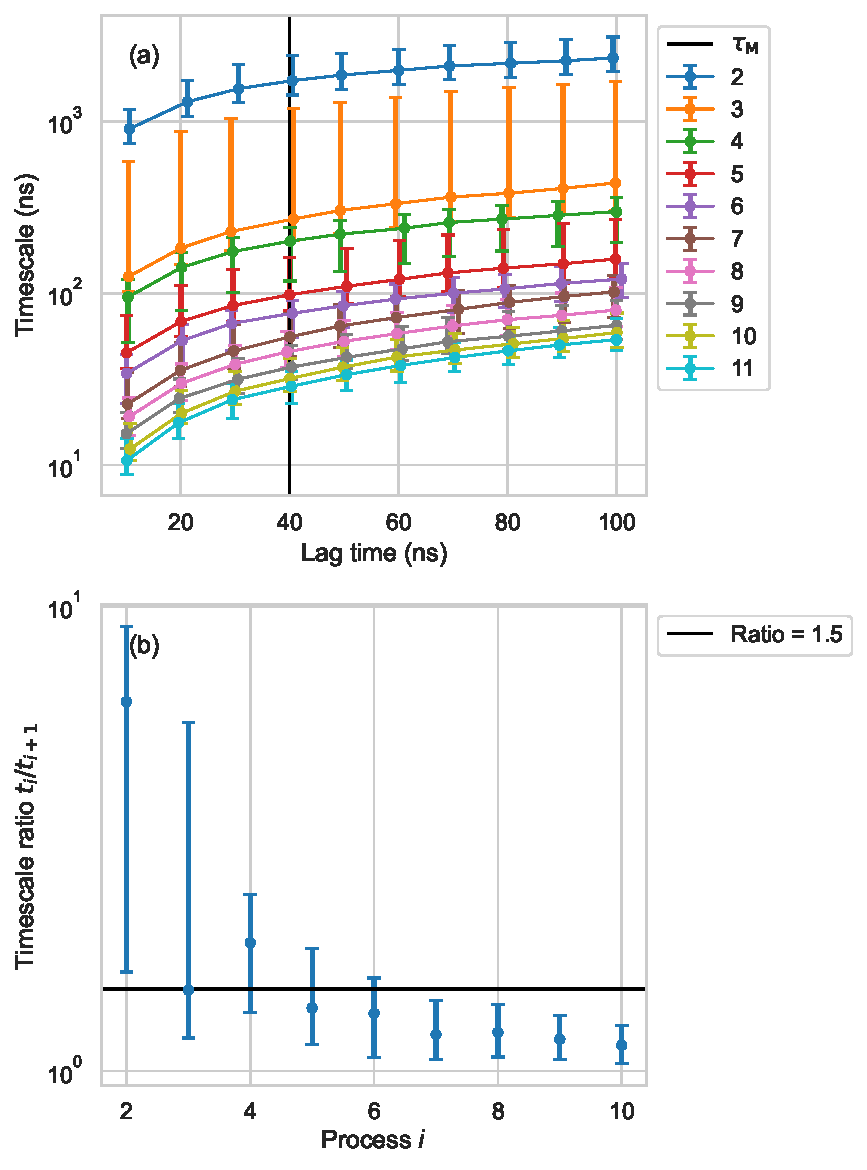
\includegraphics[height=0.65\textheight]{figures/its/bba/BBA_model_logit(dist.)_method_m2.pdf}
%     \caption{Implied timescales (panel (a)) and ratios of implied timescales at $\tau=\SI{40}{\nano\second}$ (panel (b)) for BBA model 6 (table \ref{tab:1fme_mod_defs}). Estimate and errors are the median and \SI{95}{\percent} bootstrapped quantiles respectively.}
%     \label{fig:its_bba_6}
% \end{figure}

% \begin{figure}
%     \centering
%     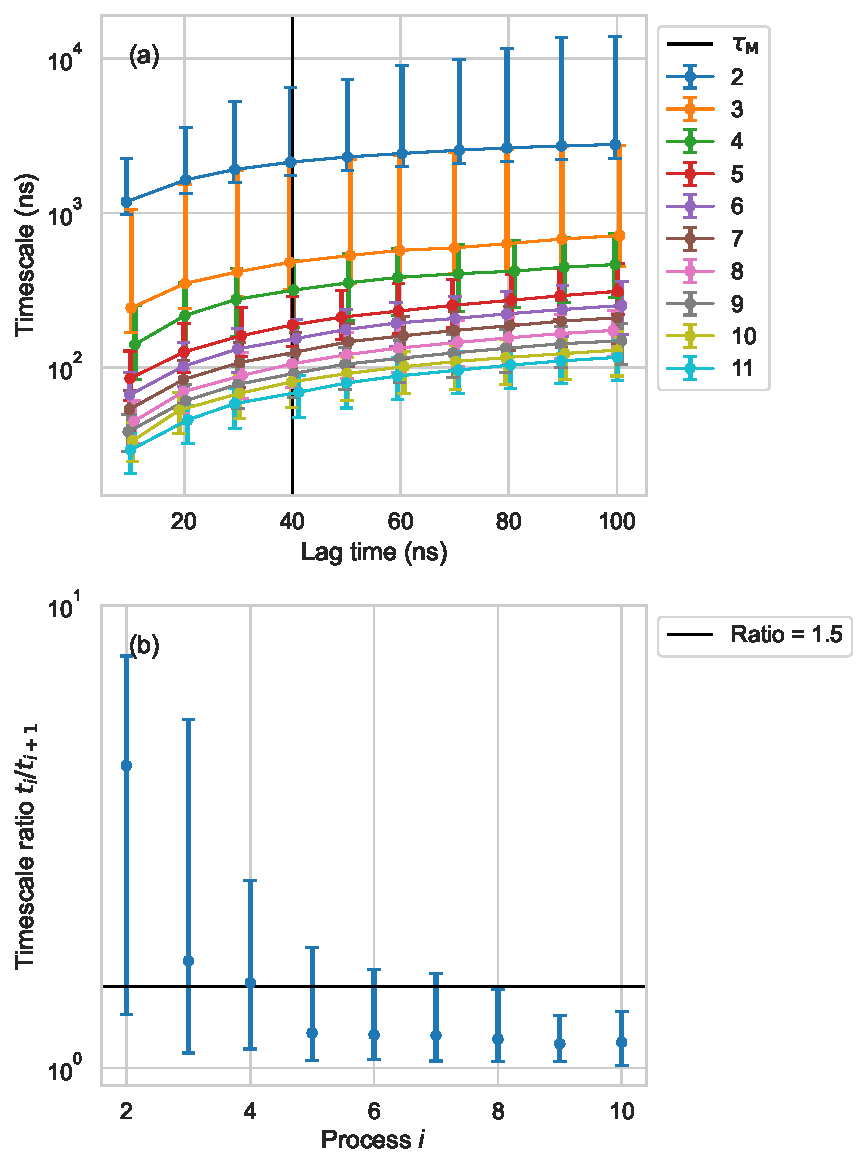
\includegraphics[height=0.65\textheight]{figures/its/bba/BBA_model_dist._method_m2.pdf}
%     \caption{Implied timescales (panel (a)) and ratios of implied timescales at $\tau=\SI{40}{\nano\second}$ (panel (b)) for BBA model 7 (table \ref{tab:1fme_mod_defs}). Estimate and errors are the median and \SI{95}{\percent} bootstrapped quantiles respectively.}
%     \label{fig:its_bba_7}
% \end{figure}

% \clearpage
% \subsection{Hyperparameter sensitivity}

% \begin{figure}[h]
%     \centering
%     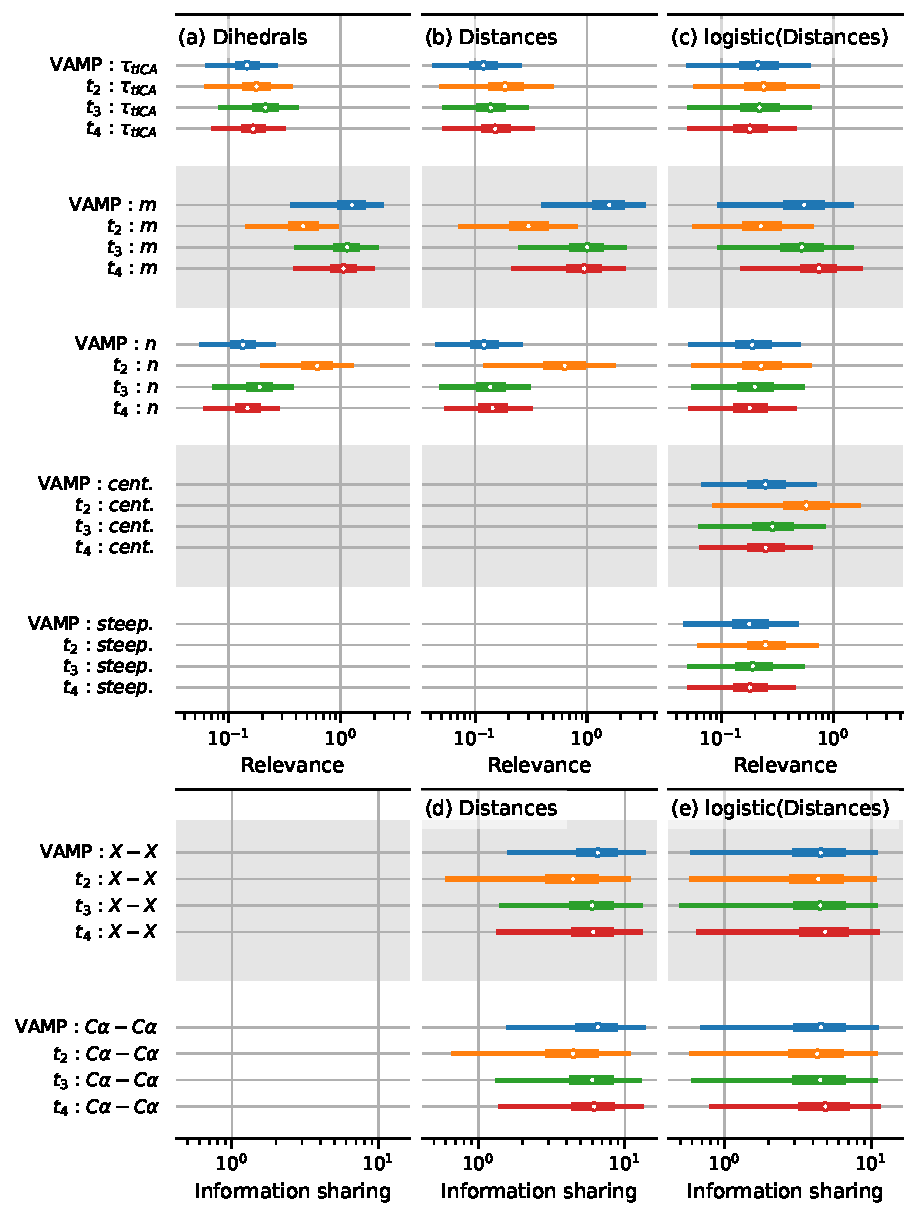
\includegraphics[height=0.7\textheight]{figures/sensitivities/1fme_sensitivity.pdf}
%     \caption{Sensitivity of hyperparameters to the VAMP-2 score with $k=4$ eigenvectors and the first three implied timescales $t_2, t_3, t_4$. Panels (a) - (c) show the relevance of the TICA lag time ($\tau_{\mathrm{tICA}}$, number of TICA dimensions, $m$, number of cluster centers, $n$ for models using the dihedrals, contact distances and logistic transformed contact distances features, respectively. Panel (c) also shows the relevance of the logistic transformation center ($cent.$) and steepness $steep.$.  Panels (d) and (e) show the degree of information sharing between hyperparameters with using the heavy atom contact scheme ($X-X$) and the alpha-Carbon contact scheme $C_{\alpha}-C_{\alpha}$. }
%     \label{fig:bba_sensitivity}
% \end{figure}

% \clearpage
% \subsection{Eigenvector comparisons}

% \begin{figure}[h]
%     \centering
%     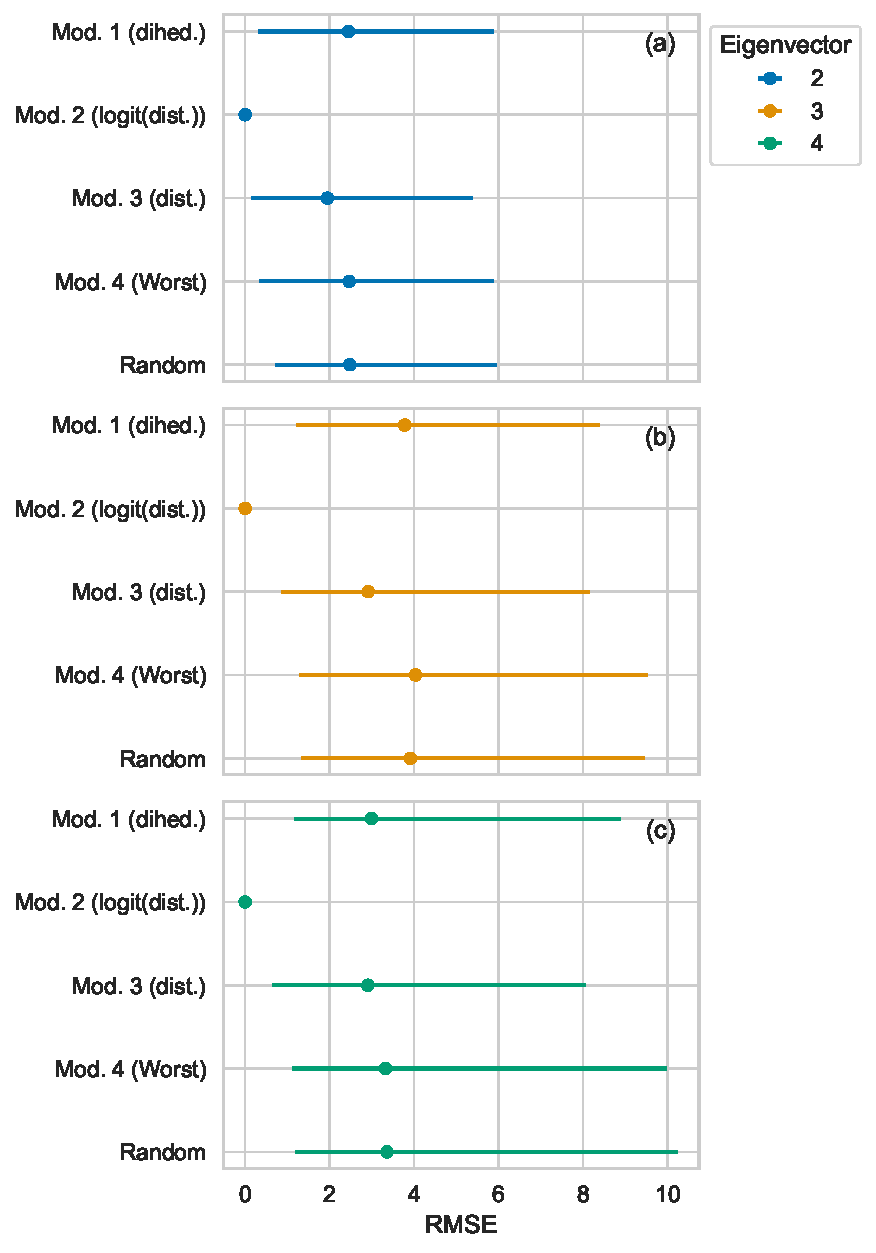
\includegraphics[width=0.7\textwidth]{figures/ev_comparisons/1fme.pdf}
%     \caption{BBA eigenvector comparisons for models 1 - 4.  Each model is compared to the best overall performing model, model 2.  Panels (a) - (c) compare eigenvectors 2 - 4 respectively. The central value and error bars are the median and \SI{95}{\percent} bootstrap quantiles respectively of the RMSE compared to model 2. }
%     \label{fig:bba_m1_ev_comparisons}
% \end{figure}

% \clearpage
% \subsection{Folded state comparisons}
% \begin{figure}[h]
%     \centering
%     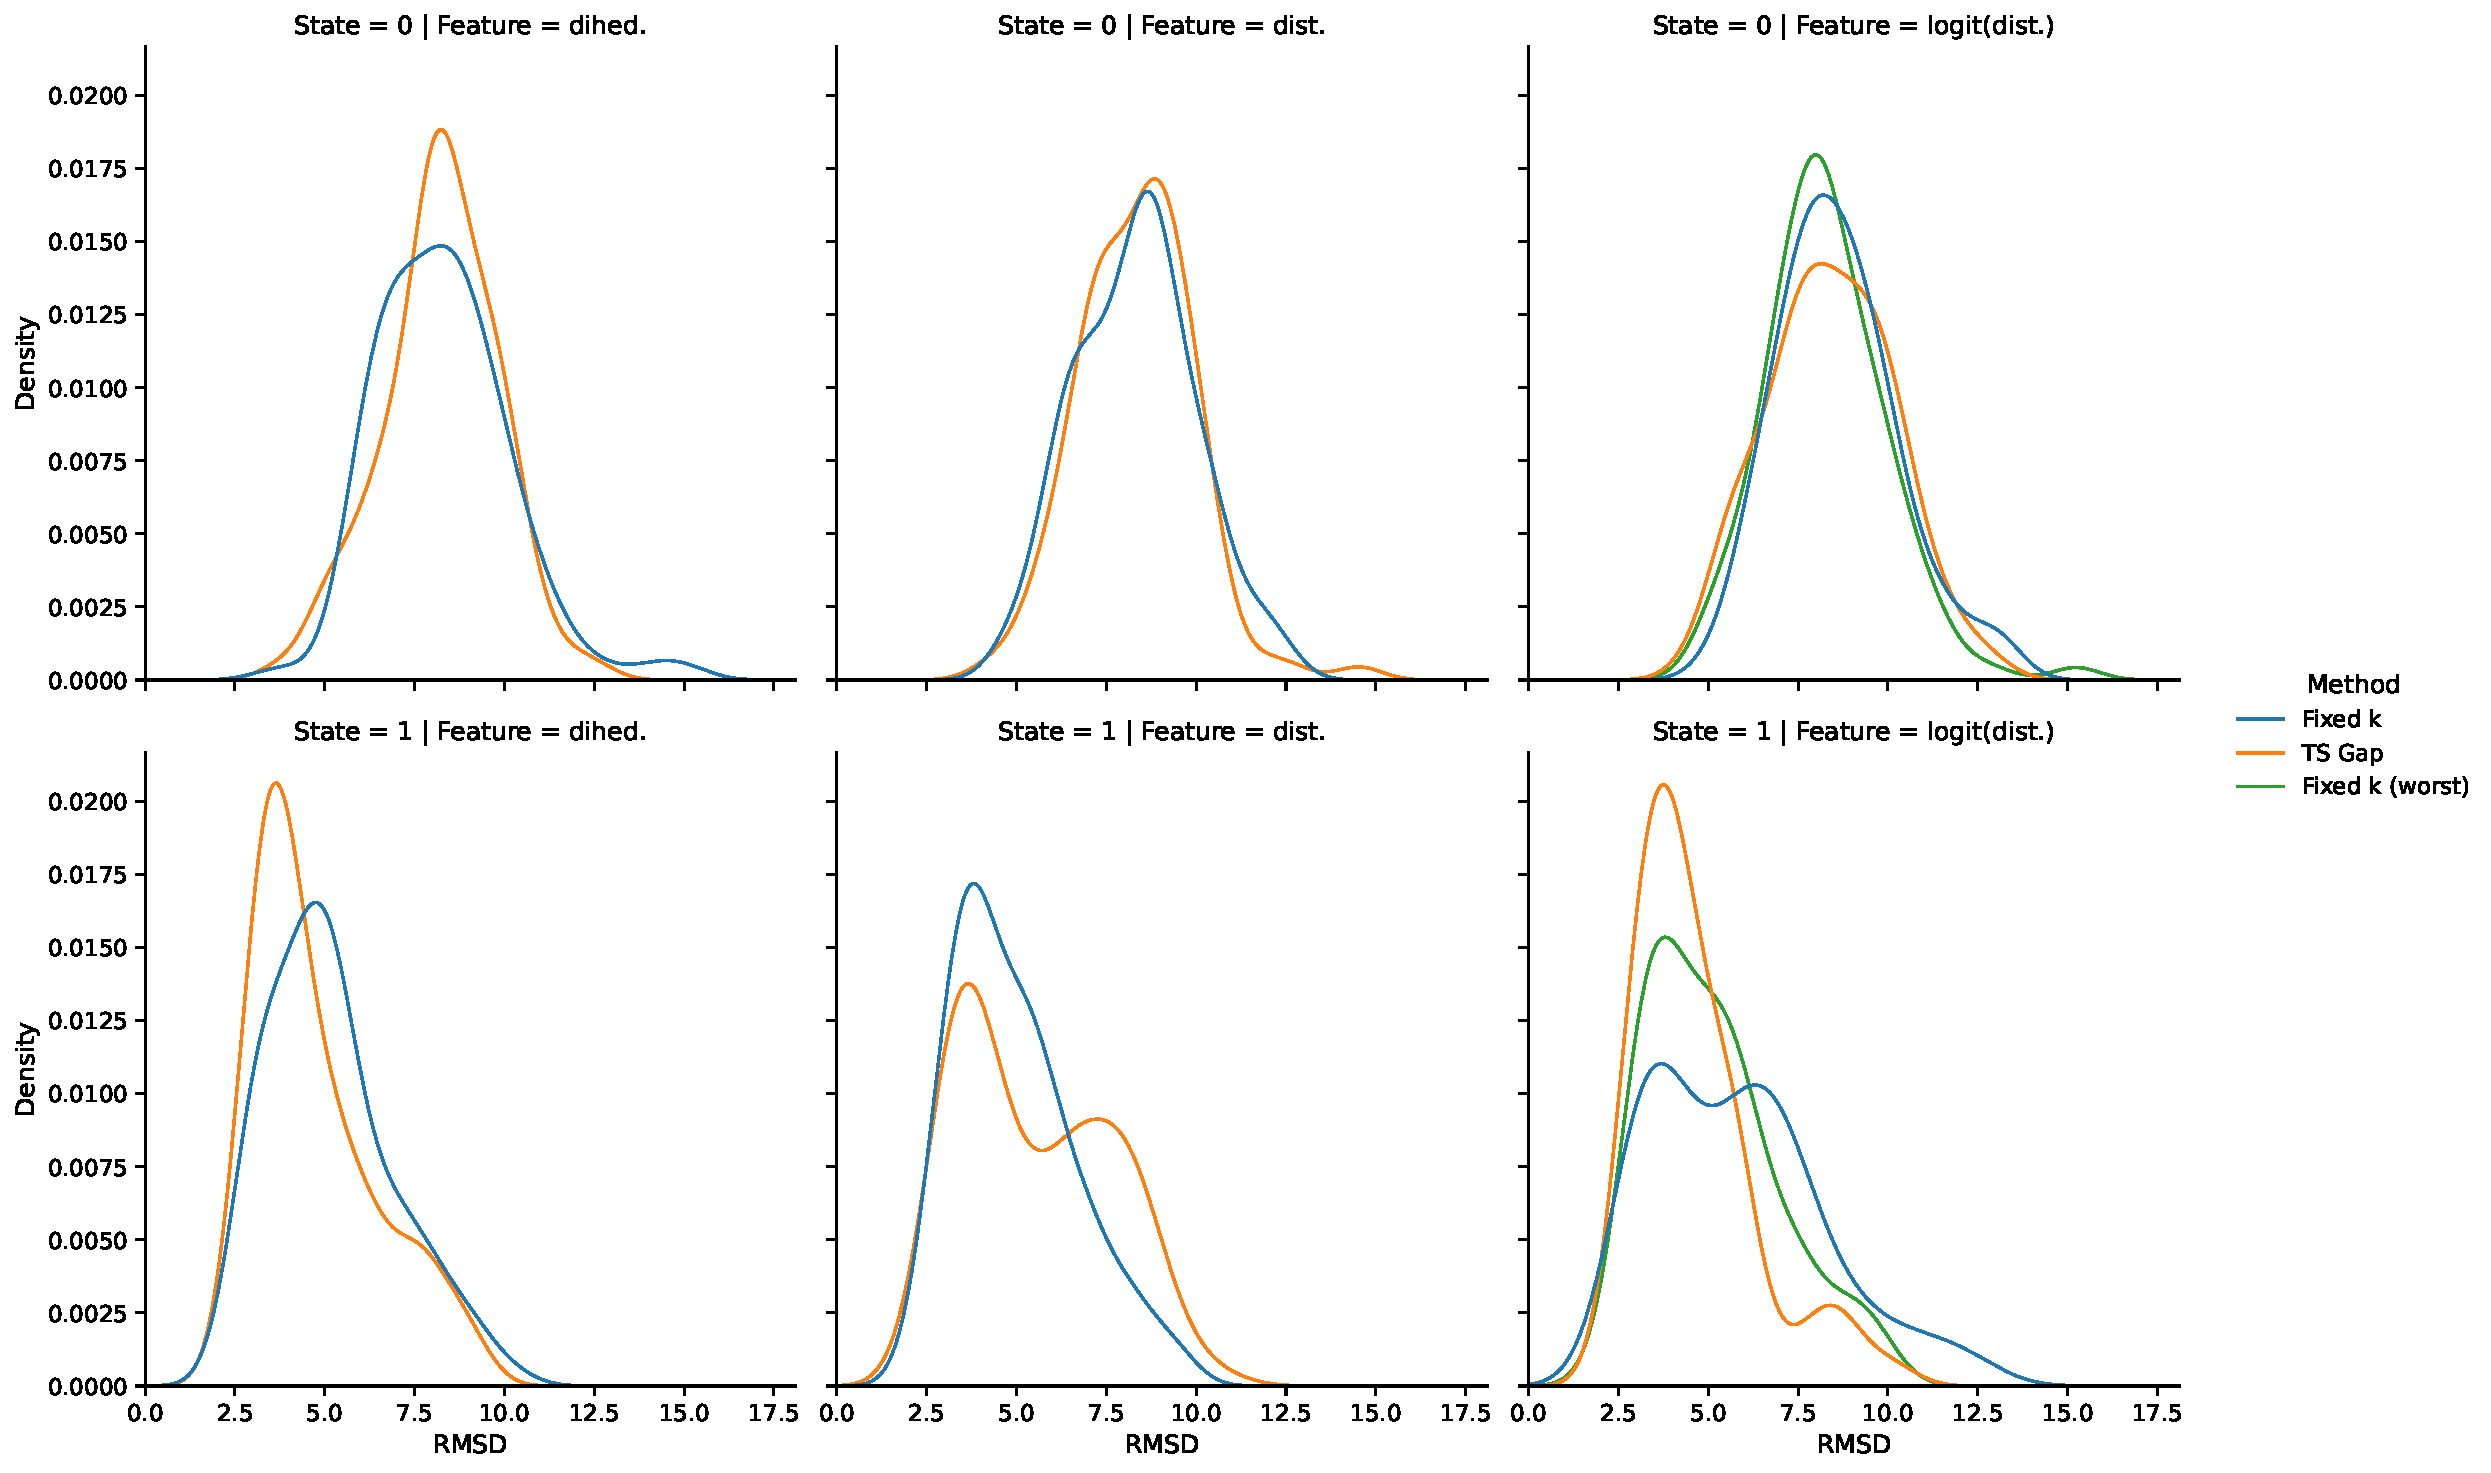
\includegraphics[width=0.9\textwidth]{figures/hmm_folded_state/BBA.pdf}
%     \caption{Comparison of metastable states to the folded state of BBA. Each model was coarse-grained with a with two state HMM. Blue lines show models 1 - 3, green line is model 4 and orange are models 5 - 7.}
%     \label{fig:bba_folded_comparisons}
% \end{figure}

% \clearpage
% \section{Villin}


% \begin{landscape}

% \begin{table}

% \begin{tabular}{llllllll}
% \toprule
% Model no. &                  1 &                  2 &                  3 &                  4 &                  5 &                  6 &                  7 \\
% \midrule
% Method                         &          Fixed $k$ &          Fixed $k$ &          Fixed $k$ &  Fixed $k$ (worst) &             TS Gap &             TS Gap &             TS Gap \\
% Lag (ns)                       &                 30 &                 30 &                 30 &                 30 &                 30 &                 30 &                 30 \\
% Feature                        &          Dihedrals &          Distances &          Distances &          Distances &          Dihedrals &          Distances &          Distances \\
% Transform                      &                  - &           Logistic &             Linear &           Logistic &                  - &           Logistic &             Linear \\
% Contact scheme                 &                  - &      Closest-Heavy &          C$\alpha$ &          C$\alpha$ &                  - &      Closest-Heavy &          C$\alpha$ \\
% Center (\si{\angstrom})        &                  - &                5.9 &                  - &                3.8 &                  - &                6.3 &                  - \\
% Steepness (\si{\per\angstrom}) &                  - &                0.2 &                  - &                3.8 &                  - &                0.4 &                  - \\
% TICA lag (ns)                  &                  6 &                 21 &                 16 &                 79 &                 13 &                 60 &                 32 \\
% TICA dimension                 &                  6 &                  5 &                  8 &                  9 &                  2 &                  2 &                  2 \\
% Num. clusters                  &                458 &                296 &                291 &                300 &                 19 &                 52 &                117 \\
% $k_{\mathrm{fixed}}$           &                  3 &                  3 &                  3 &                  3 &                  3 &                  3 &                  3 \\
% $k_{\mathrm{gap}}$             &                  3 &                  3 &                  3 &                  2 &                  3 &                  3 &                  3 \\
% VAMP-2(k=2)                    &  1.93, [1.84-1.96] &  1.90, [1.85-1.94] &  1.92, [1.86-1.95] &  1.47, [1.40-1.52] &  1.93, [1.80-1.96] &  1.88, [1.83-1.93] &  1.91, [1.85-1.95] \\
% VAMP-2(k=3)                    &  2.76, [2.65-2.80] &  2.74, [2.63-2.78] &  2.77, [2.68-2.81] &  1.50, [1.42-1.65] &  2.72, [2.57-2.76] &  2.72, [2.60-2.76] &  2.76, [2.66-2.79] \\
% VAMP-2(k=4)                    &  3.20, [3.02-3.34] &  3.22, [3.02-3.40] &  3.29, [3.12-3.47] &  1.53, [1.45-1.74] &  2.85, [2.68-3.07] &  2.95, [2.77-3.10] &  3.06, [2.88-3.22] \\
% \bottomrule
% \end{tabular}

% \caption{\textsc{Summary of comparator models for Villin.} Models 1 - 4 are selected using a fixed number of processes ($k_{\mathrm{fixed}}$) in the VAMP2 score, and are the best performing models for each feature (1 -3) and the worst performing model overall (4).  Models 5 - 7 are the best performing models for each feature after consideration of the timescale gap. The number of processes is used to calculate this is $k_{\mathrm{gap}}$.}
% \label{tab:2f4k_mod_defs}
% \end{table}
% \end{landscape}

% \clearpage
% \subsection{VAMP-2 scores}

% \begin{figure}[h]
%     \centering
%     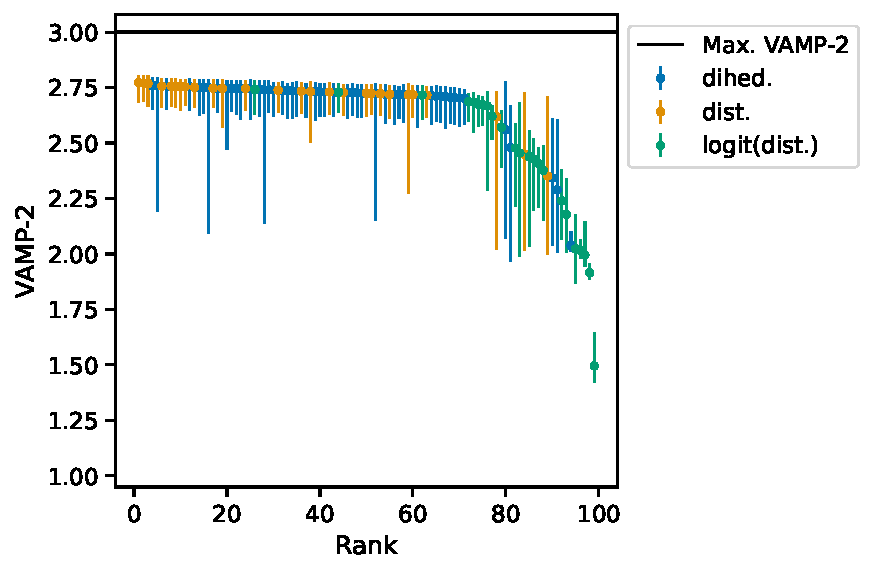
\includegraphics[width=0.9\textwidth]{figures/vamp_scores/Villin_vamp_scores_ranked.pdf}
%     \caption{Villin hyperparameter trial scores using the VAMP-2 with $k=3$ eigenvectors. Trials are ranked using the median of the VAMP-2 score, errors shown are the \SI{95}{\percent} quantiles of 100 bootstrapped smaples.}
%     \label{fig:villin_vamp_fixed_k}
% \end{figure}

% \clearpage
% \begin{figure}
%     \centering
%     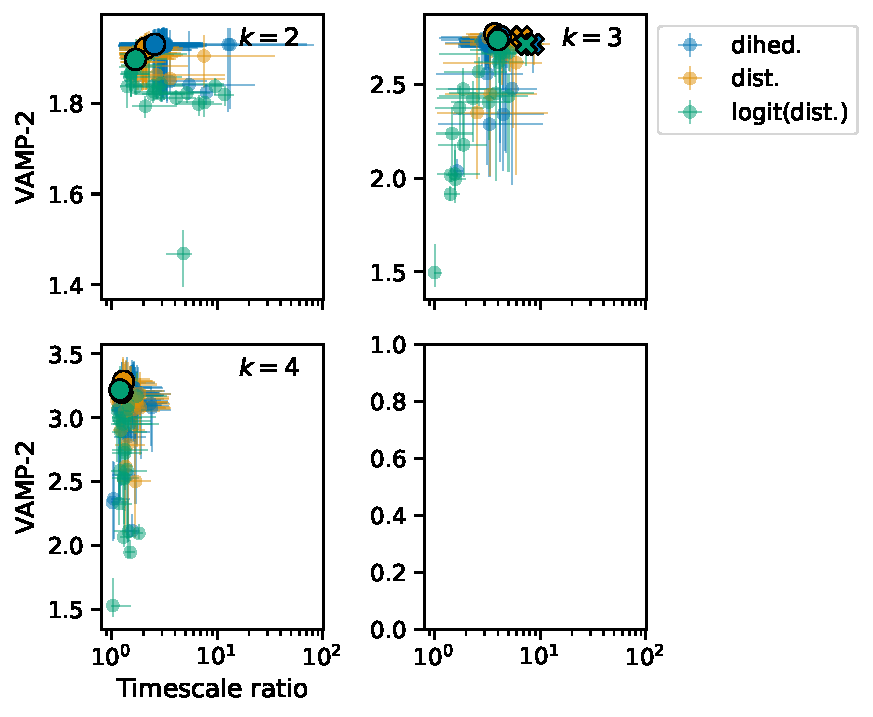
\includegraphics[width=0.9\textwidth]{figures/vamp_scores/Villin_vamp_vs_gap.pdf}
%     \caption{Villin hyperparameter trial scores and implied timescale gaps.  Each panel shows the VAMP-2 score with $k$ eigenvectors against the ratio of implied timescales $t_{k}/t_{k+1}$. Large coloured disks show the models selected using $k=3$ eigenvectors (models 1 - 3 in table \ref{tab:2f4k_mod_defs}).  Crosses show the models selected using the timescale ratio and VAMP-2 scores (models 5 - 7 in table \ref{tab:2f4k_mod_defs}).}
%     \label{fig:villin_vamp_var_k}
% \end{figure}


% \clearpage
% \subsection{Chapman-Kolmogorov Tests}

% \begin{figure}[h]
%     \centering
%     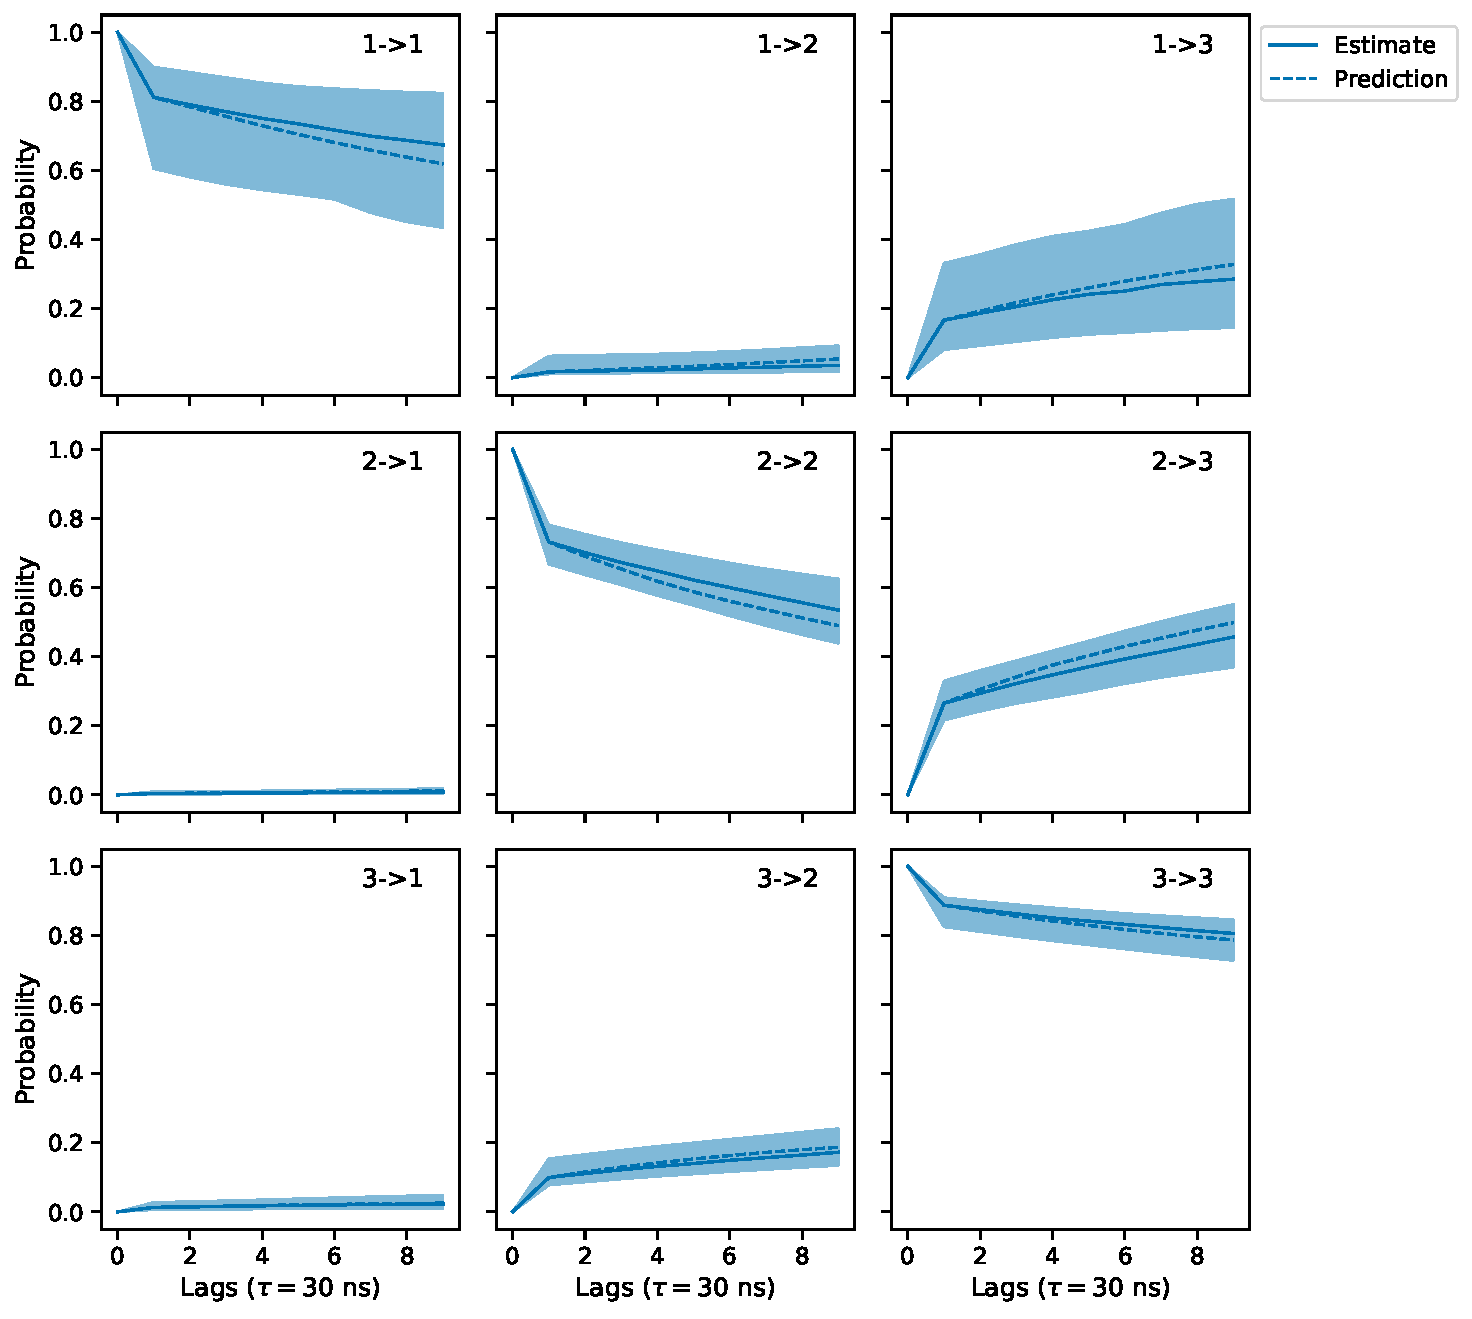
\includegraphics[height=0.4\textheight]{figures/cktests/villin/m1_dihed_hpix67_cktest.pdf}
%     \caption{Chapman Kolmogorov test for Villin model 1 (table \ref{tab:2f4k_mod_defs}). Estimate and errors are the median and \SI{95}{\percent} bootstrapped quantiles respectively.}
%     \label{fig:cktest_villin_1}
% \end{figure}

% \begin{figure}
%     \centering
%     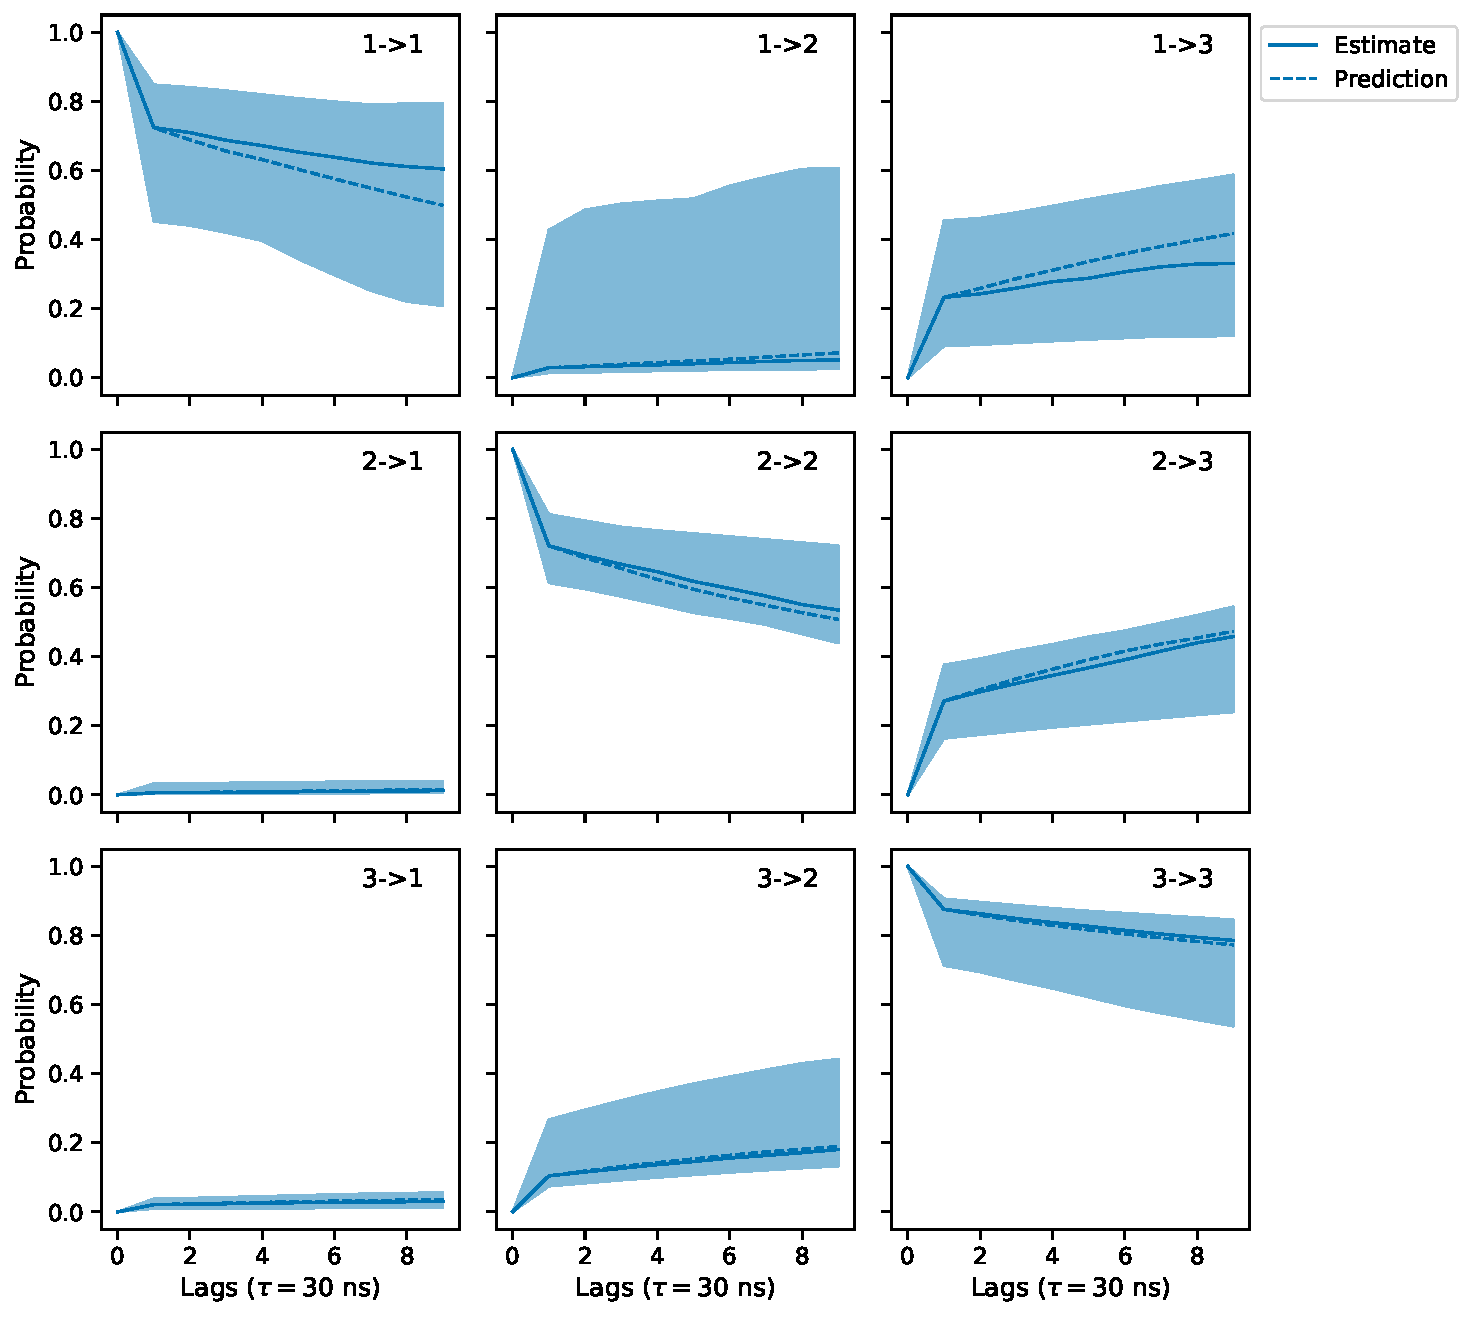
\includegraphics[height=0.4\textheight]{figures/cktests/villin/m1_logit(dist)_hpix84_cktest.pdf}
%     \caption{Chapman Kolmogorov test for Villin model 2 (table \ref{tab:2f4k_mod_defs}). Estimate and errors are the median and \SI{95}{\percent} bootstrapped quantiles respectively. }
%     \label{fig:cktest_villin_2}
% \end{figure}

% \begin{figure}
%     \centering
%     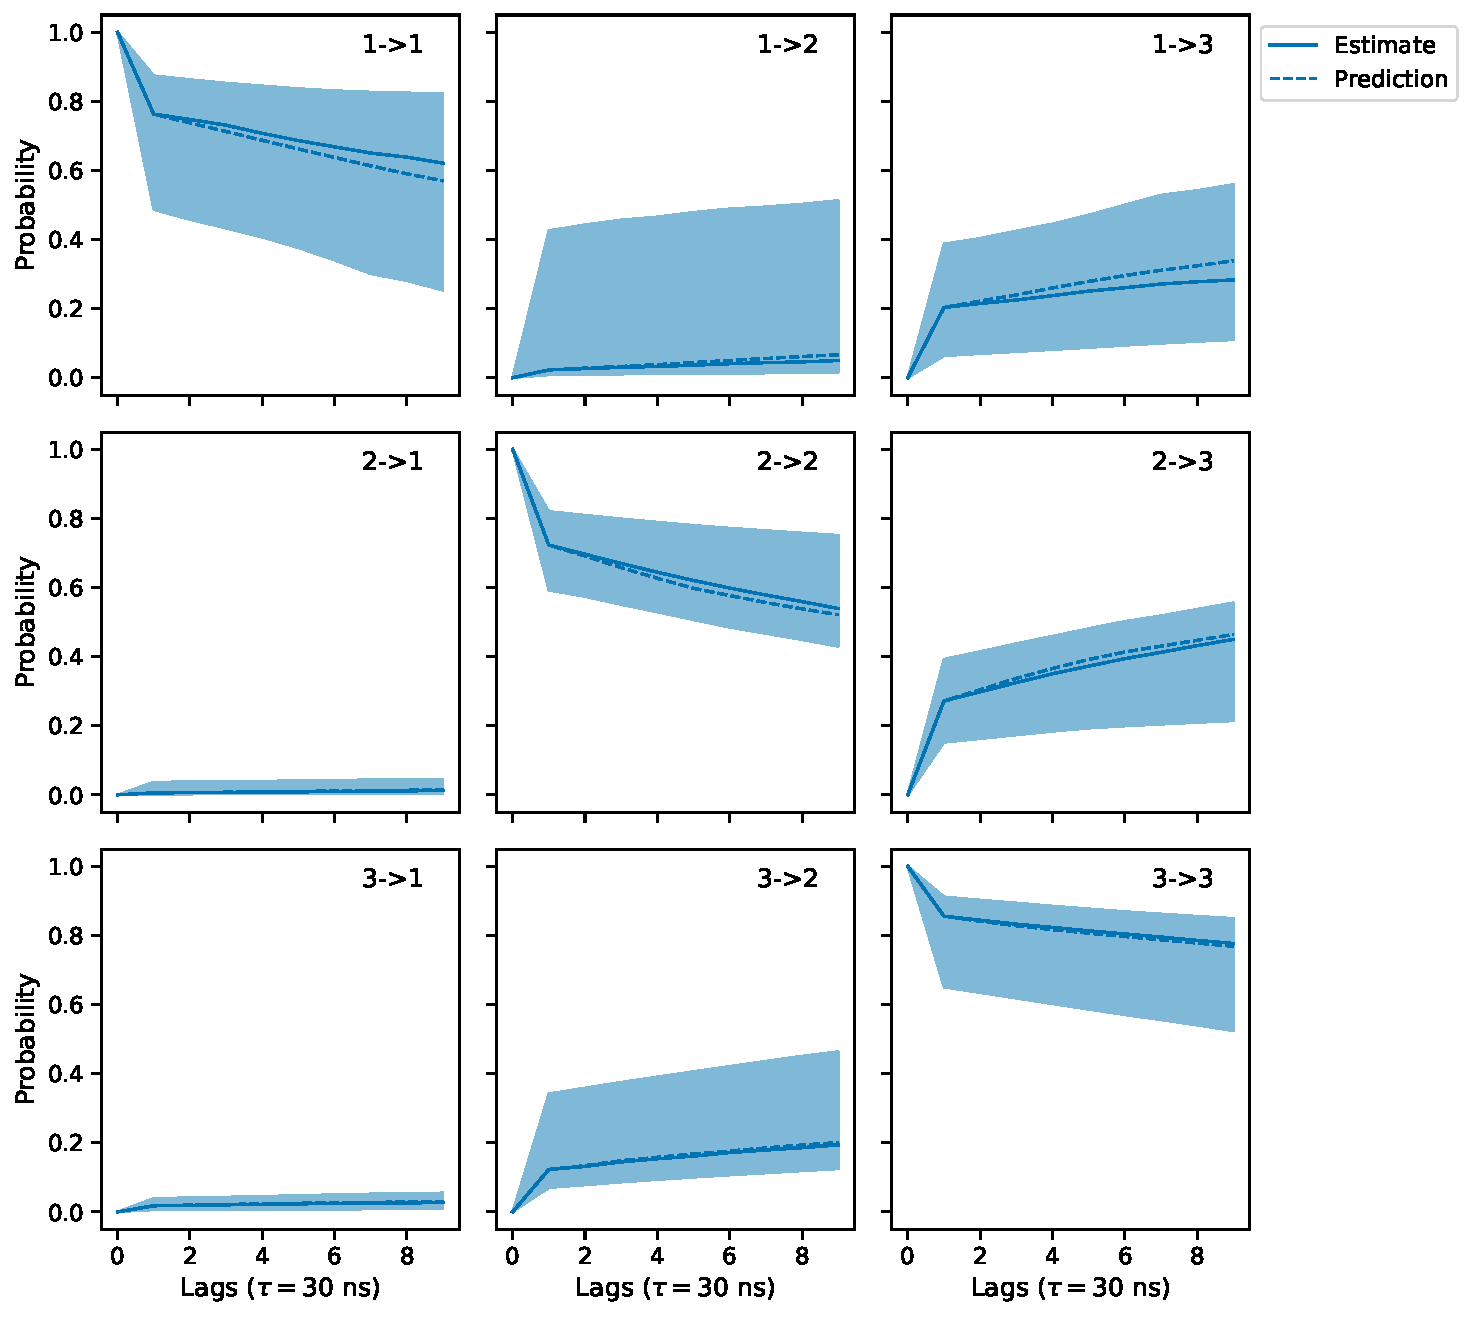
\includegraphics[height=0.4\textheight]{figures/cktests/villin/m1_dist_hpix56_cktest.pdf}
%     \caption{Chapman Kolmogorov test for Villin model 3 (table \ref{tab:2f4k_mod_defs}). Estimate and errors are the median and \SI{95}{\percent} bootstrapped quantiles respectively.}
%     \label{fig:cktest_villin_3}
% \end{figure}

% \begin{figure}
%     \centering
%     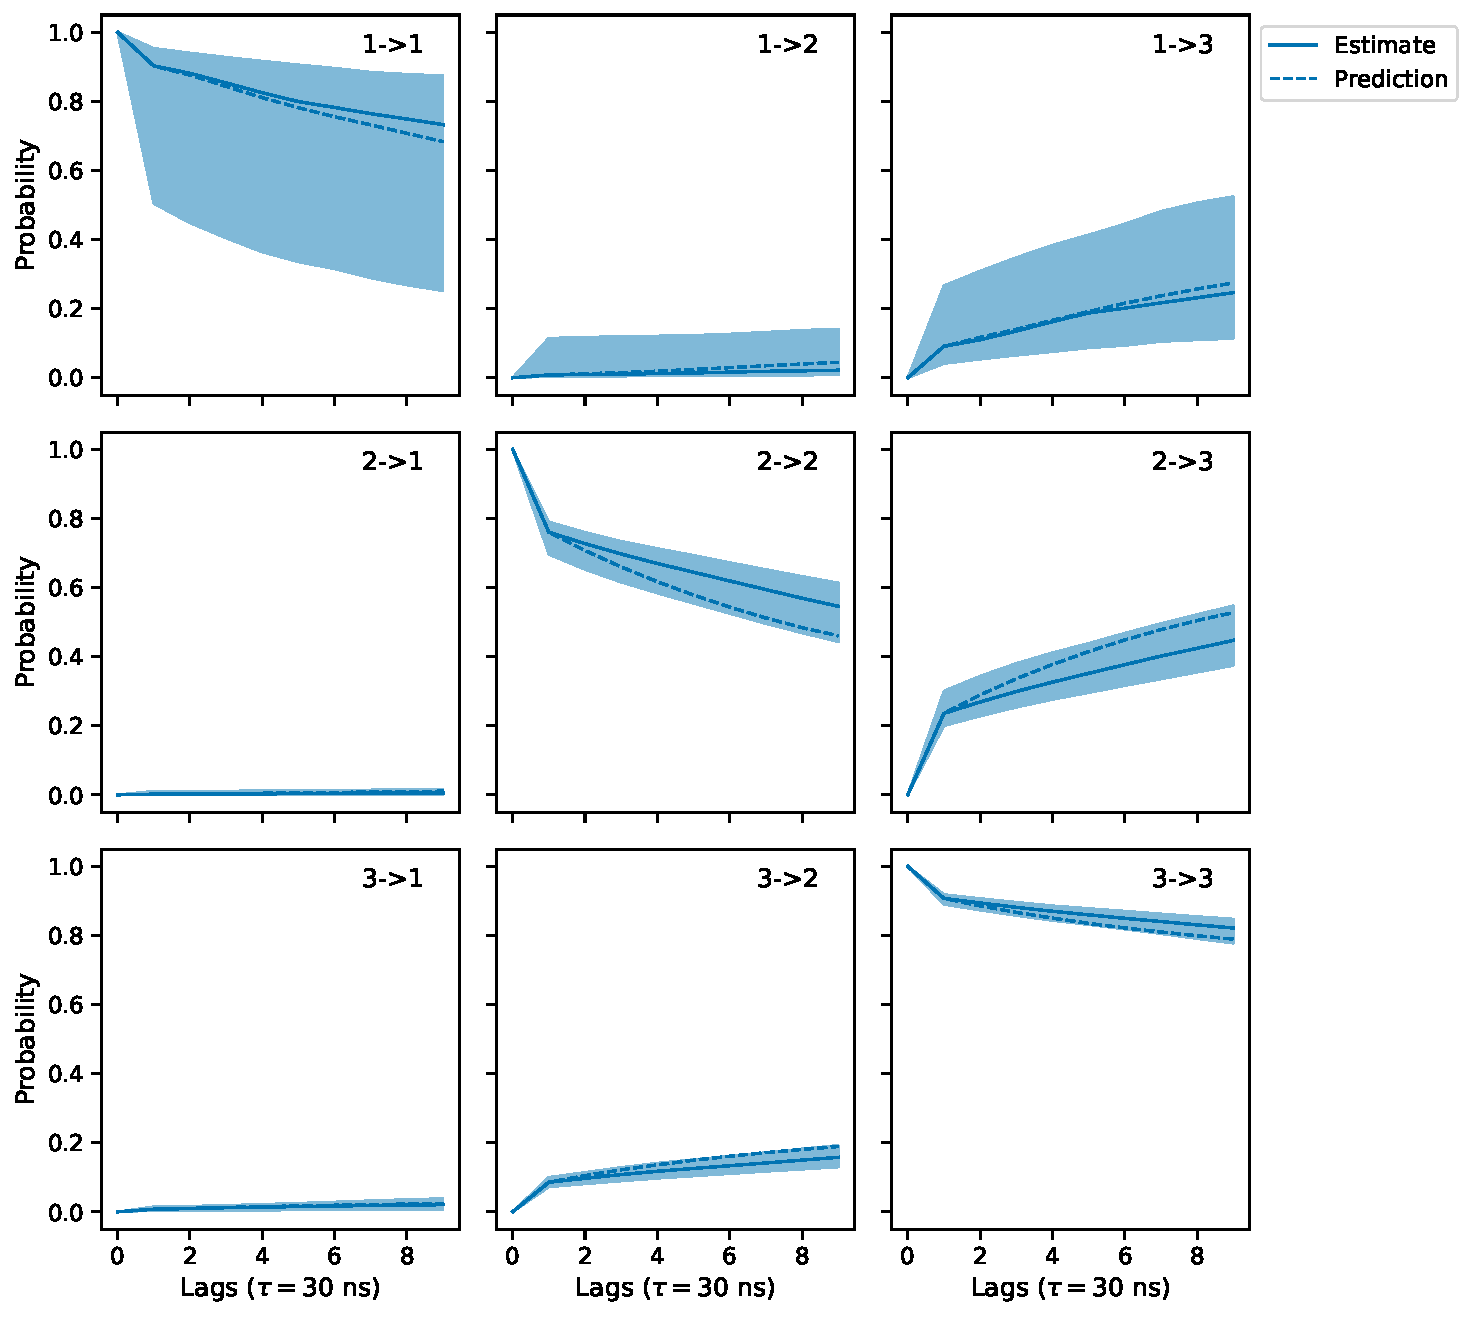
\includegraphics[height=0.4\textheight]{figures/cktests/villin/m2_dihed_hpix17_cktest.pdf}
%     \caption{Chapman Kolmogorov test for Villin model 5 (table \ref{tab:2f4k_mod_defs}). Estimate and errors are the median and \SI{95}{\percent} bootstrapped quantiles respectively.}
%     \label{fig:cktest_villin_5}
% \end{figure}

% \begin{figure}
%     \centering
%     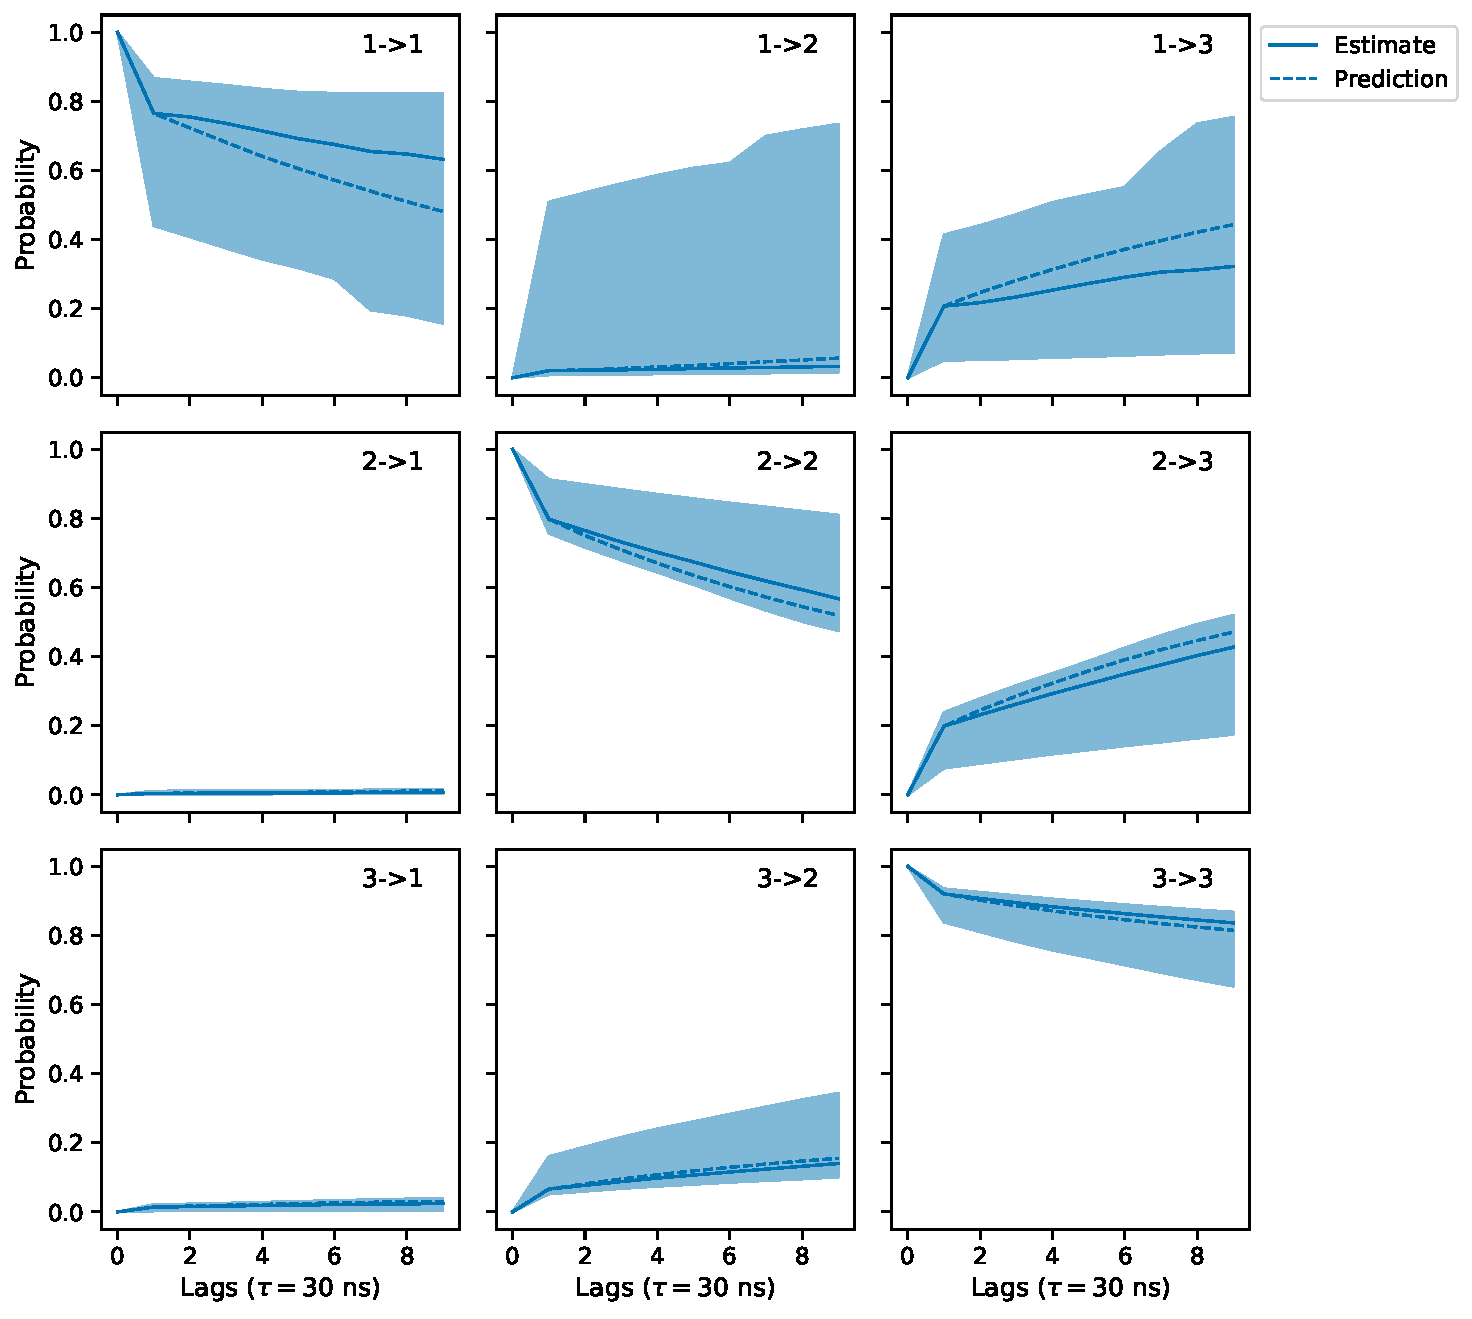
\includegraphics[height=0.4\textheight]{figures/cktests/villin/m2_logit(dist)_hpix14_cktest.pdf}
%     \caption{Chapman Kolmogorov test for Villin model 6 (table \ref{tab:2f4k_mod_defs}). Estimate and errors are the median and \SI{95}{\percent} bootstrapped quantiles respectively.}
%     \label{fig:cktest_villin_6}
% \end{figure}

% \begin{figure}
%     \centering
%     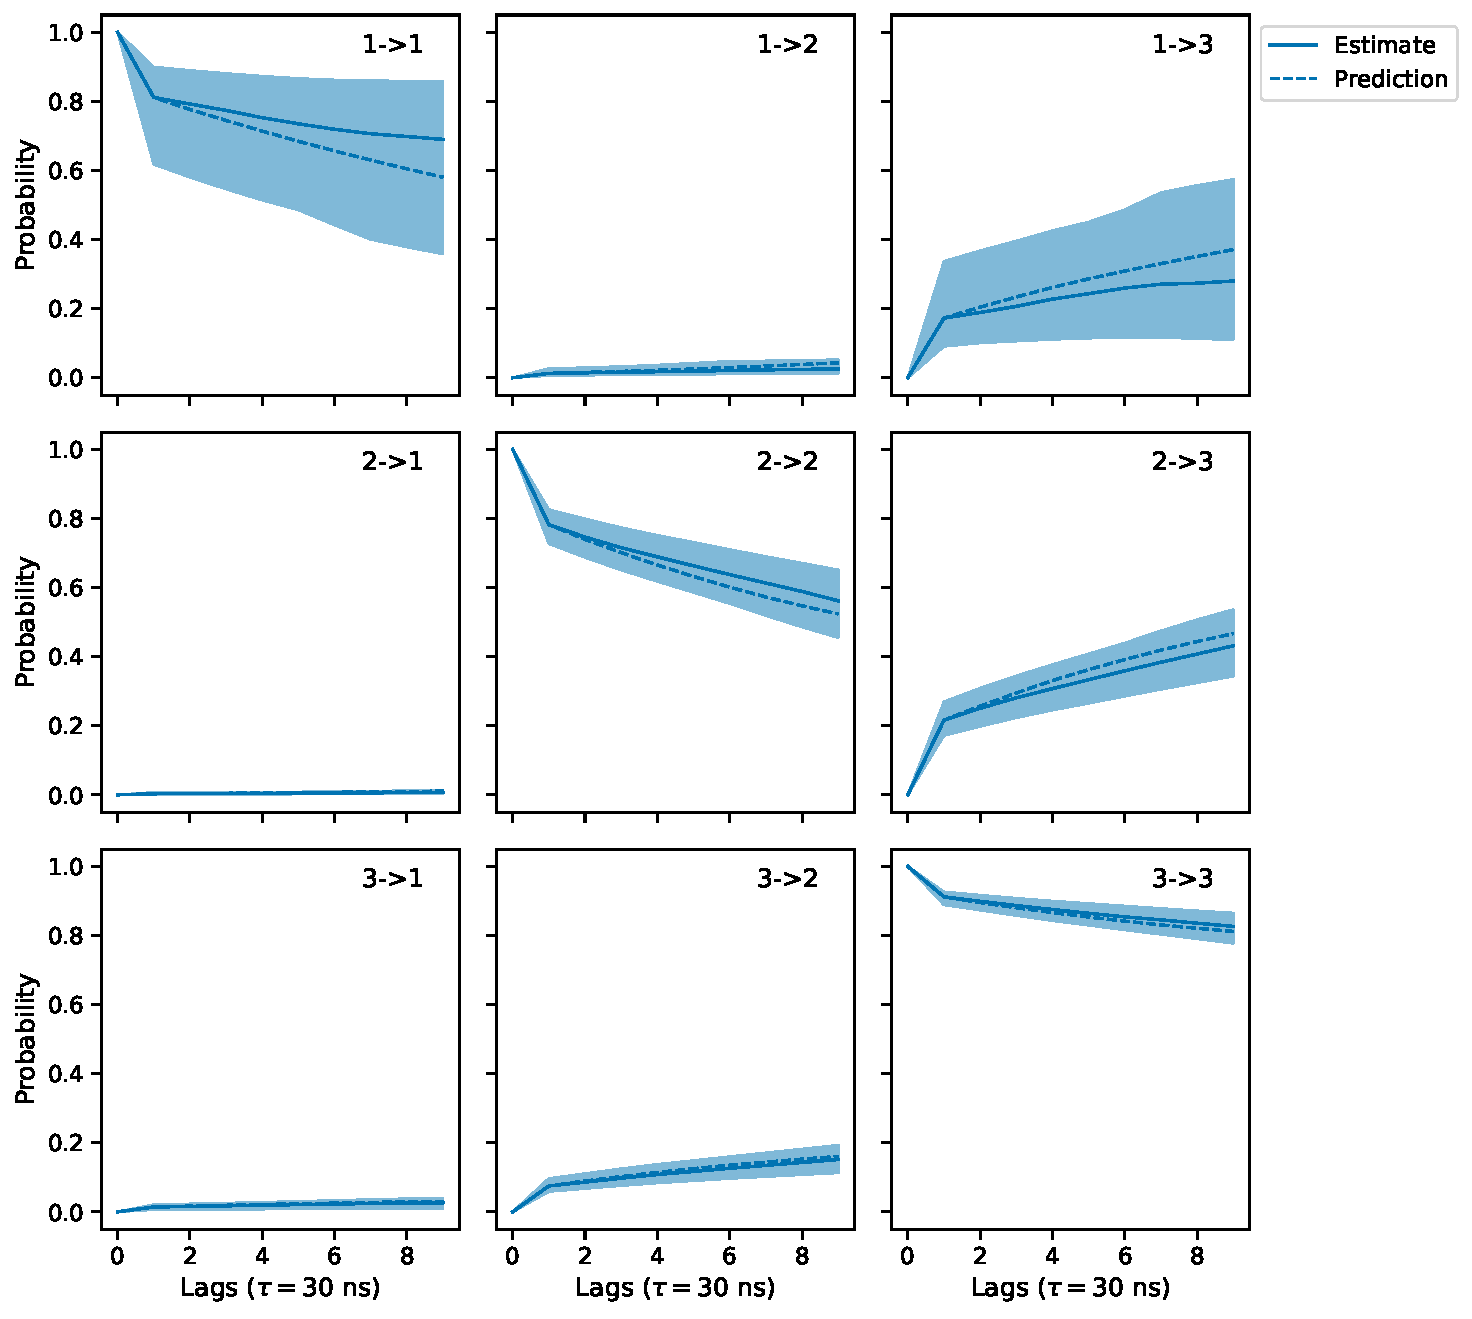
\includegraphics[height=0.4\textheight]{figures/cktests/villin/m2_dist_hpix79_cktest.pdf}
%     \caption{Chapman Kolmogorov test for Villin model 7 (table \ref{tab:2f4k_mod_defs}). Estimate and errors are the median and \SI{95}{\percent} bootstrapped quantiles respectively.}
%     \label{fig:cktest_villin_7}
% \end{figure}

% \clearpage
% \subsection{Implied timescales and separation of timescales}

% \begin{figure}[h]
%     \centering
%     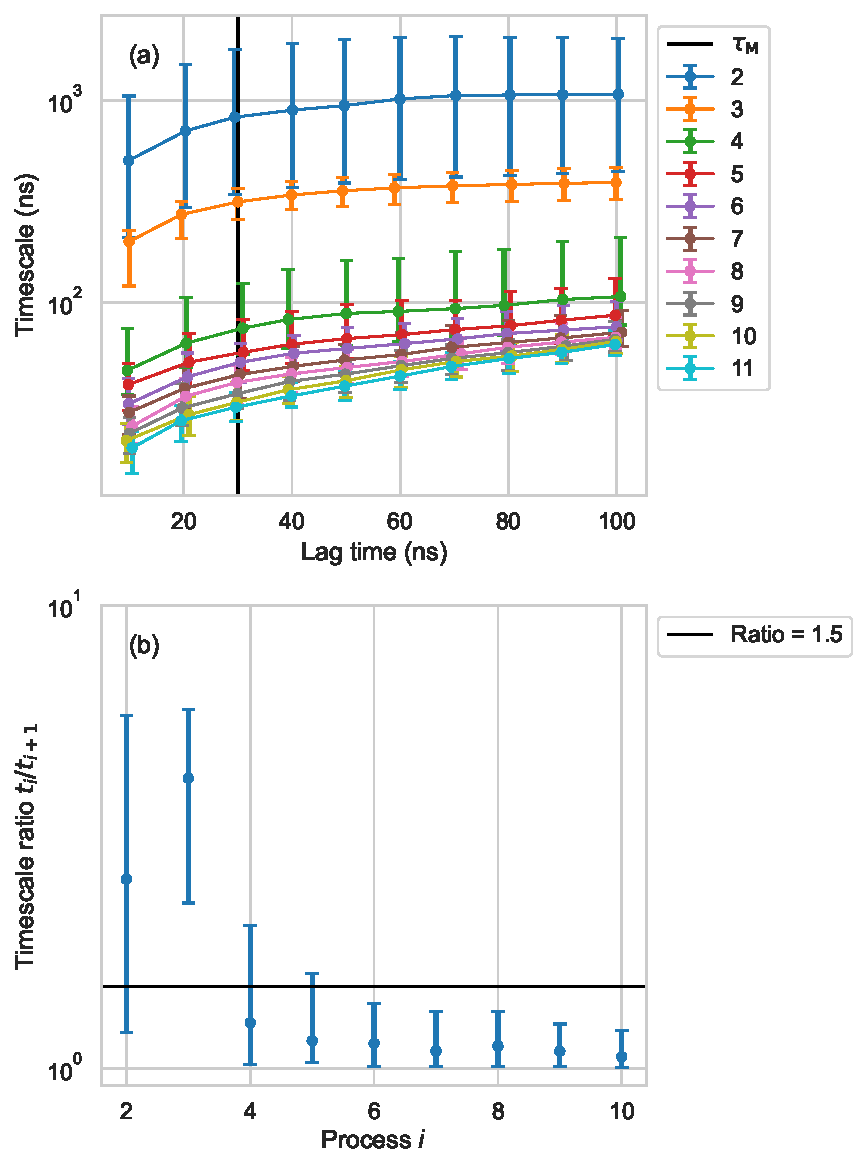
\includegraphics[height=0.65\textheight]{figures/its/villin/Villin_model_dihed._method_m1.pdf}
%     \caption{Implied timescales (panel (a)) and ratios of implied timescales at $\tau=\SI{20}{\nano\second}$ (panel (b)) for Villin model 1 (table \ref{tab:2f4k_mod_defs}). Estimate and errors are the median and \SI{95}{\percent} bootstrapped quantiles respectively.}
%     \label{fig:its_villin_1}
% \end{figure}

% \begin{figure}
%     \centering
%     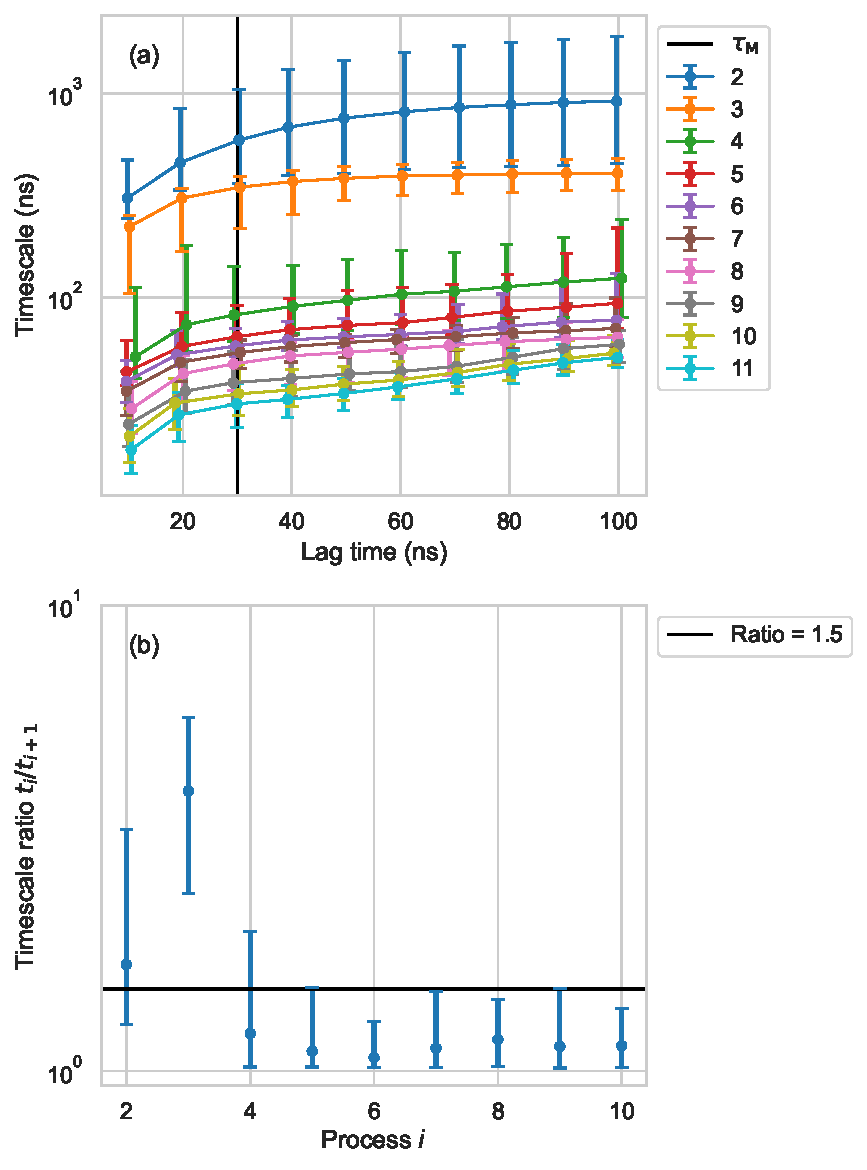
\includegraphics[height=0.65\textheight]{figures/its/villin/Villin_model_logit(dist.)_method_m1.pdf}
%     \caption{Implied timescales (panel (a)) and ratios of implied timescales at $\tau=\SI{20}{\nano\second}$ (panel (b)) for Villin model 2 (table \ref{tab:2f4k_mod_defs}). Estimate and errors are the median and \SI{95}{\percent} bootstrapped quantiles respectively.}
%     \label{fig:its_villin_2}
% \end{figure}

% \begin{figure}
%     \centering
%     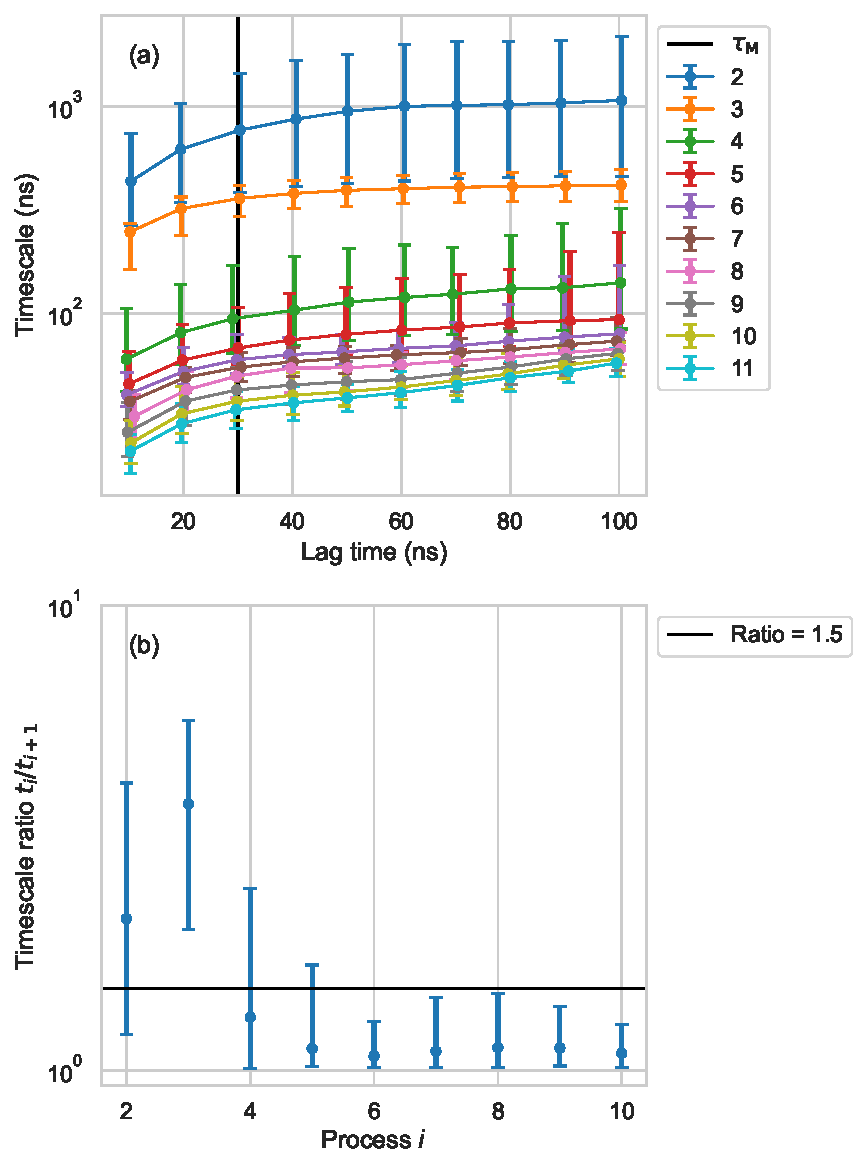
\includegraphics[height=0.65\textheight]{figures/its/villin/Villin_model_dist._method_m1.pdf}
%     \caption{Implied timescales (panel (a)) and ratios of implied timescales at $\tau=\SI{20}{\nano\second}$ (panel (b)) for Villin model 3 (table \ref{tab:2f4k_mod_defs}). Estimate and errors are the median and \SI{95}{\percent} bootstrapped quantiles respectively.}
%     \label{fig:its_villin_3}
% \end{figure}

% \begin{figure}
%     \centering
%     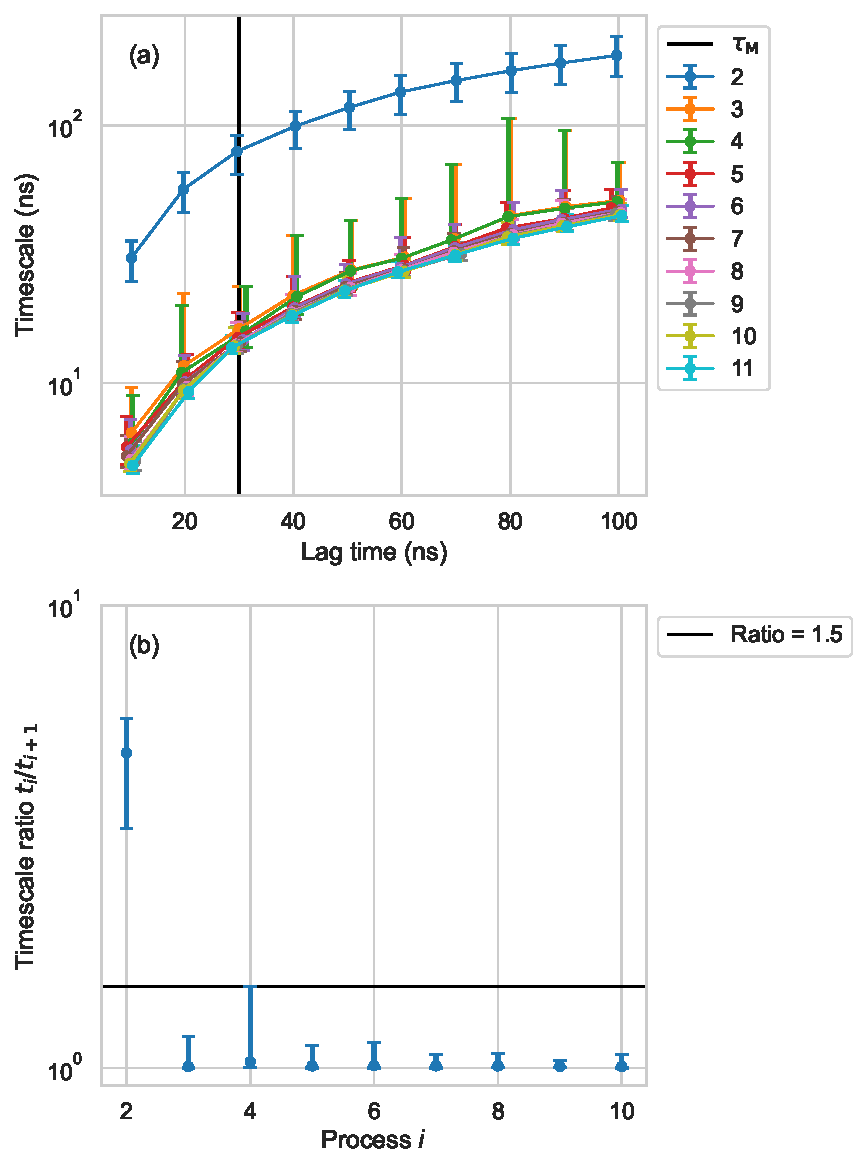
\includegraphics[height=0.65\textheight]{figures/its/villin/Villin_model_logit(dist.)_method_m3.pdf}
%     \caption{Implied timescales (panel (a)) and ratios of implied timescales at $\tau=\SI{20}{\nano\second}$ (panel (b)) for Villin model 4 (table \ref{tab:2f4k_mod_defs}). Estimate and errors are the median and \SI{95}{\percent} bootstrapped quantiles respectively.}
%     \label{fig:its_villin_4}
% \end{figure}

% \begin{figure}
%     \centering
%     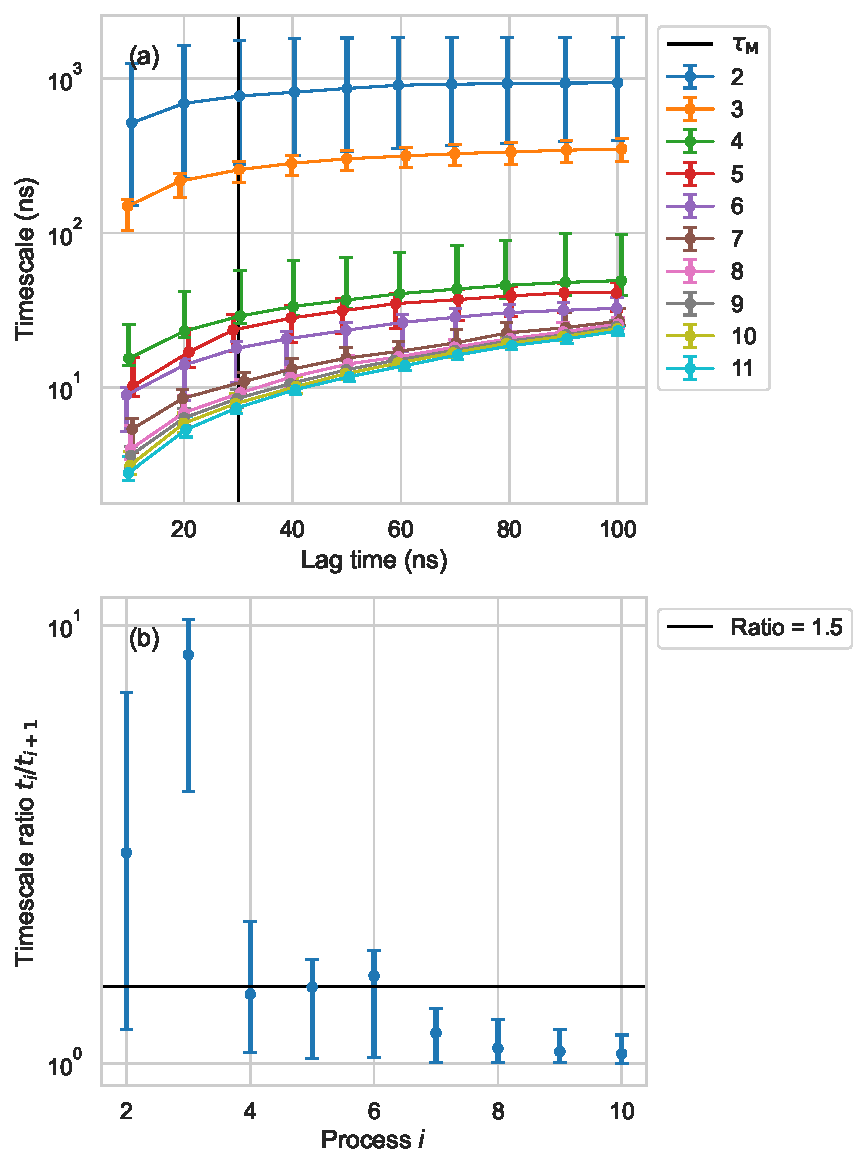
\includegraphics[height=0.65\textheight]{figures/its/villin/Villin_model_dihed._method_m2.pdf}
%     \caption{Implied timescales (panel (a)) and ratios of implied timescales at $\tau=\SI{20}{\nano\second}$ (panel (b)) for Villin model 5 (table \ref{tab:2f4k_mod_defs}). Estimate and errors are the median and \SI{95}{\percent} bootstrapped quantiles respectively.}
%     \label{fig:its_villin_5}
% \end{figure}



% \begin{figure}
%     \centering
%     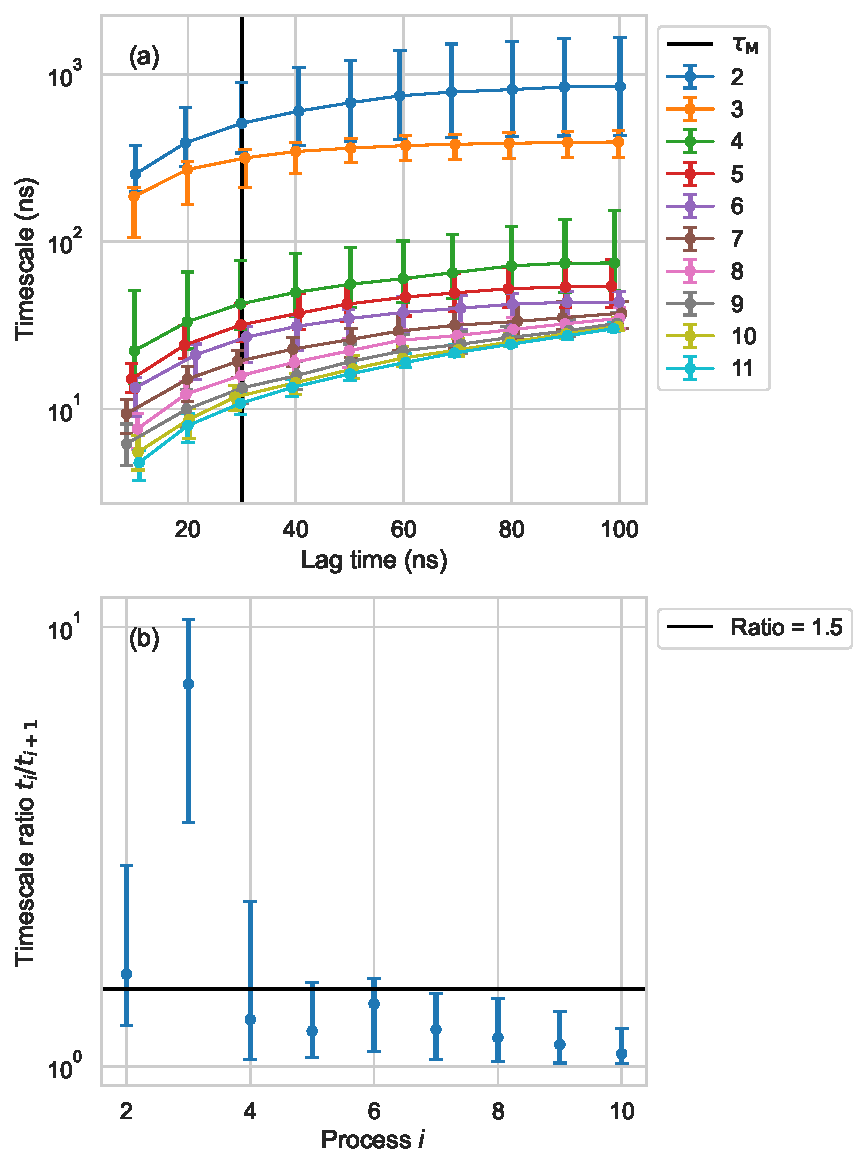
\includegraphics[height=0.65\textheight]{figures/its/villin/Villin_model_logit(dist.)_method_m2.pdf}
%     \caption{Implied timescales (panel (a)) and ratios of implied timescales at $\tau=\SI{20}{\nano\second}$ (panel (b)) for Villin model 6 (table \ref{tab:2f4k_mod_defs}). Estimate and errors are the median and \SI{95}{\percent} bootstrapped quantiles respectively.}
%     \label{fig:its_villin_6}
% \end{figure}

% \begin{figure}
%     \centering
%     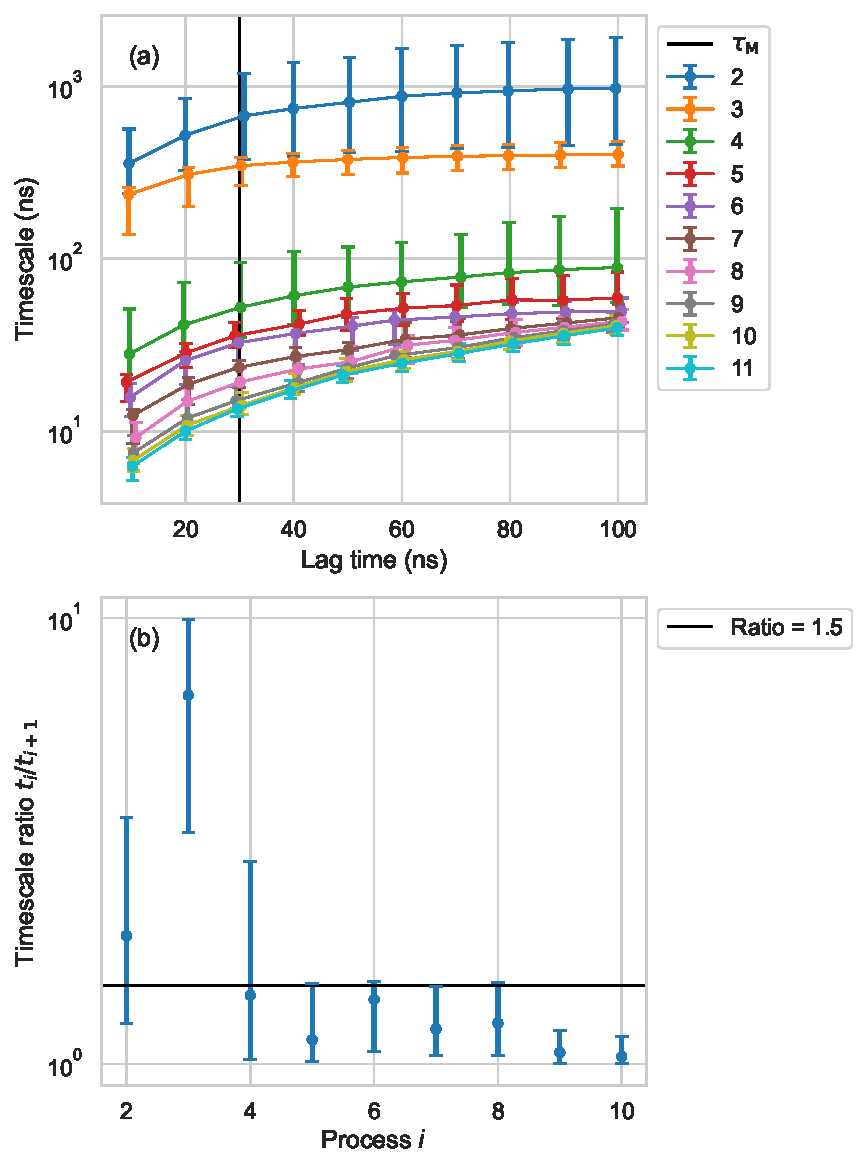
\includegraphics[height=0.65\textheight]{figures/its/villin/Villin_model_dist._method_m2.pdf}
%     \caption{Implied timescales (panel (a)) and ratios of implied timescales at $\tau=\SI{20}{\nano\second}$ (panel (b)) for Villin model 7 (table \ref{tab:2f4k_mod_defs}). Estimate and errors are the median and \SI{95}{\percent} bootstrapped quantiles respectively.}
%     \label{fig:its_villin_7}
% \end{figure}

% \clearpage
% \subsection{Hyperparameter sensitivity}

% \begin{figure}[h]
%     \centering
%     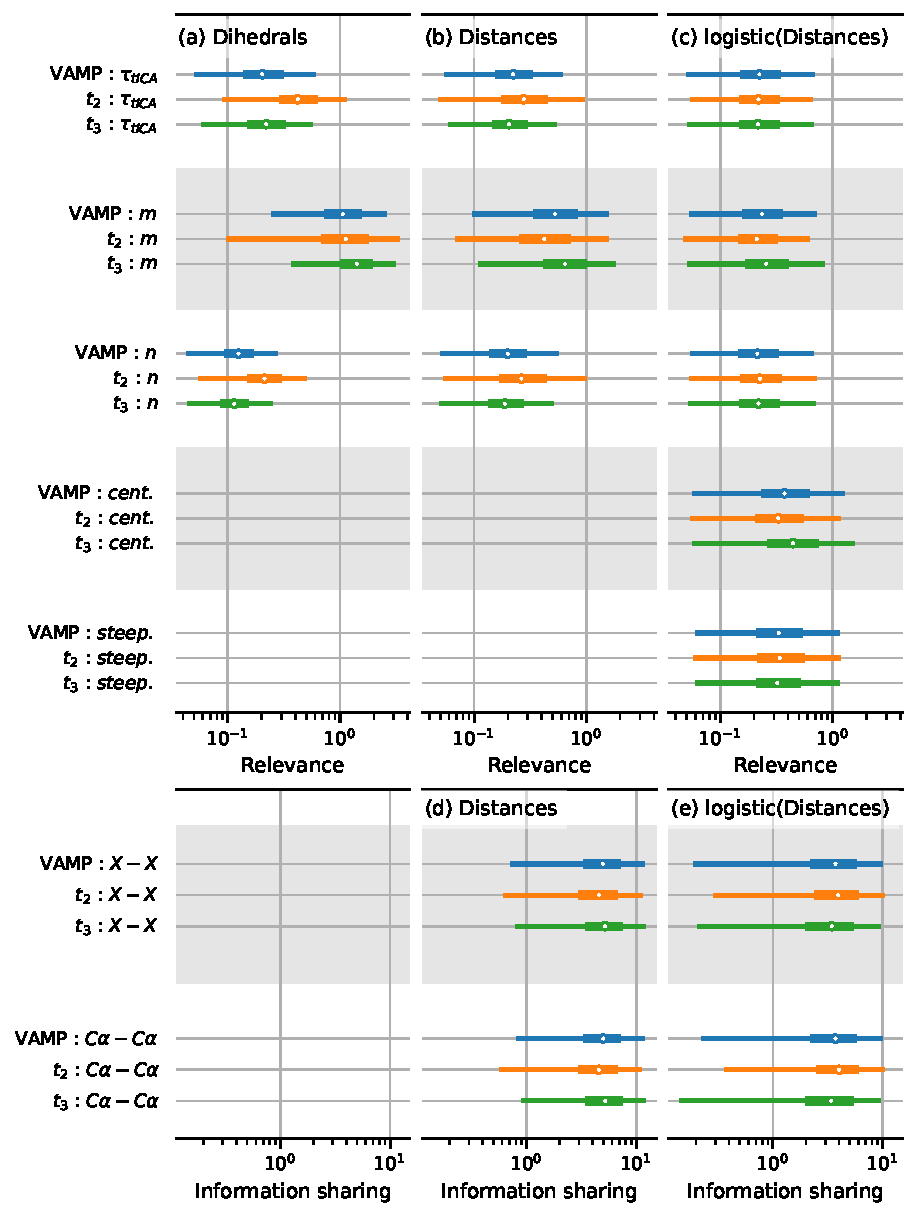
\includegraphics[height=0.7\textheight]{figures/sensitivities/2f4k_sensitivity.pdf}
%     \caption{Sensitivity of hyperparameters to the VAMP-2 score with $k=3$ eigenvectors ($VAMP$) and the first three implied timescales ($t_2, t_3, t_4$). Panels (a) - (c) show the relevance of the TICA lag time ($\tau_{\mathrm{tICA}}$, number of TICA dimensions, $m$, number of cluster centers, $n$ for models using the dihedrals, contact distances and logistic transformed contact distances features, respectively. Panel (c) also shows the relevance of the logistic transformation center ($cent.$) and steepness $steep.$.  Panels (d) and (e) show the degree of information sharing between hyperparameters with using the heavy atom contact scheme ($X-X$) and the alpha-Carbon contact scheme $C_{\alpha}-C_{\alpha}$. }
%     \label{fig:villin_sensitivity}
% \end{figure}

% \clearpage
% \subsection{Eigenvector comparisons}

% \begin{figure}[h]
%     \centering
%     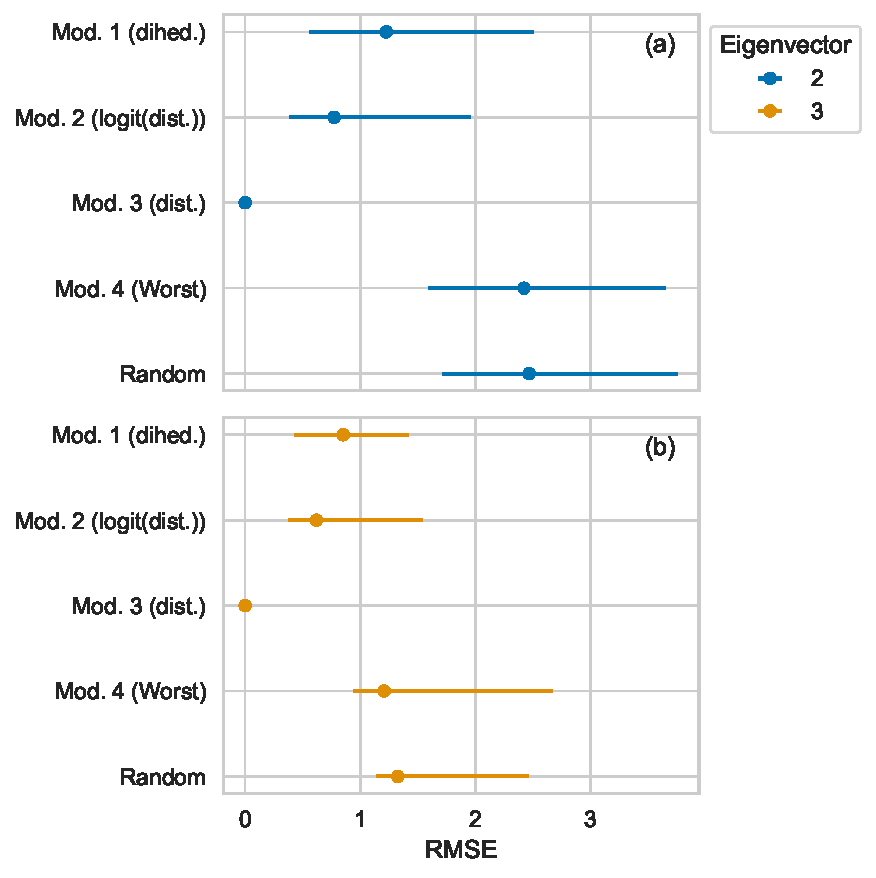
\includegraphics[width=0.7\textwidth]{figures/ev_comparisons/2f4k.pdf}
%     \caption{Villin eigenvector comparisons for models 1 - 4.  Each model is compared to the best overall performing model, model 3.  Panels (a) - (c) compare eigenvectors 2 - 4 respectively. The central value and error bars are the median and \SI{95}{\percent} bootstrap quantiles respectively of the RMSE compared to model 3. }
%     \label{fig:villin_m1_ev_comparisons}
% \end{figure}

% \clearpage
% \subsection{Folded state comparisons}
% \begin{figure}[h]
%     \centering
%     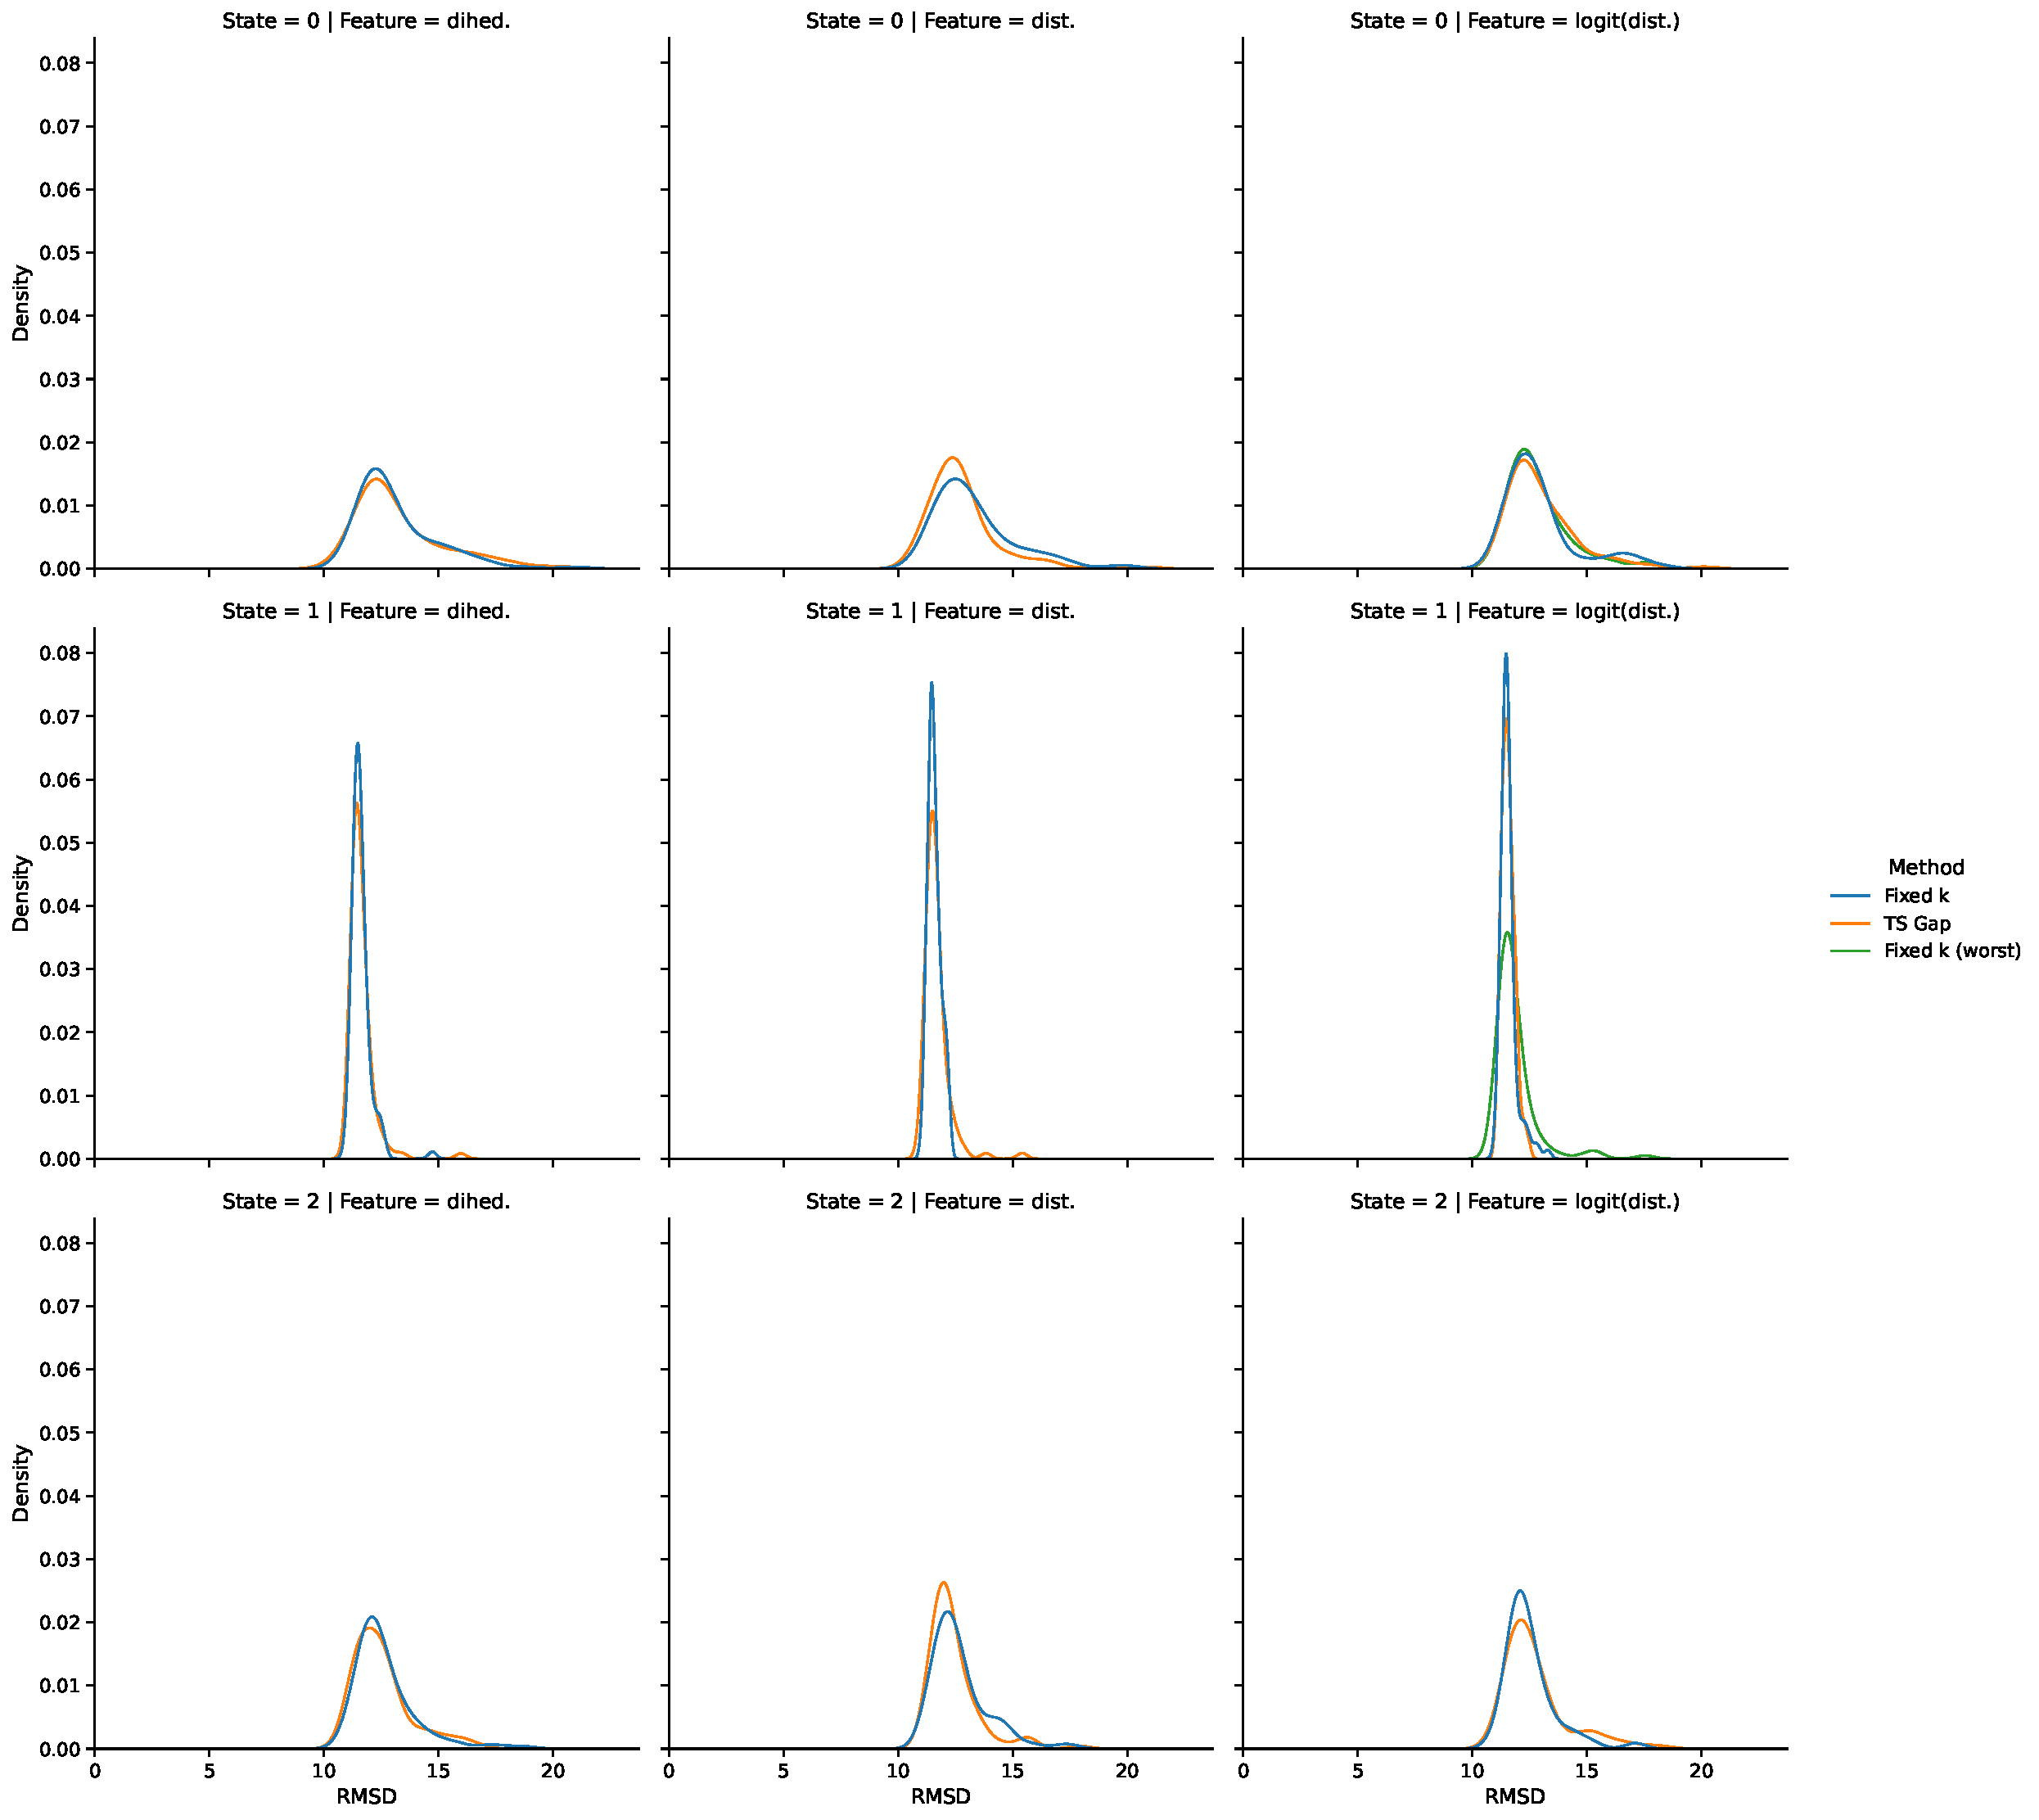
\includegraphics[width=0.9\textwidth]{figures/hmm_folded_state/Villin.pdf}
%     \caption{Comparison of metastable states to the folded state of Villin. Each model was coarse-grained with a with two state HMM. Blue lines show models 1 - 3, green line is model 4 and orange are models 5 - 7.}
%     \label{fig:villin_m1_ev_comparisons}
% \end{figure}

\end{document}
